\documentclass[11pt,a4paper]{article}

\usepackage[utf8]{inputenc}
\usepackage[T1]{fontenc}
\usepackage[french]{babel}
\usepackage{lmodern}
\usepackage{geometry}
\usepackage{graphicx}
\usepackage{booktabs}
\usepackage{longtable}
\usepackage{array}
\usepackage{float}
\usepackage{hyperref}
\usepackage{xcolor}
\usepackage{enumitem}
\usepackage{caption}
\usepackage{setspace}
\usepackage{fancyhdr}
\usepackage{titlesec}

\geometry{margin=2.5cm}
\definecolor{uniblue}{RGB}{22,52,92}
\definecolor{unigrey}{RGB}{90,98,110}
\hypersetup{
    colorlinks=true,
    linkcolor=uniblue,
    urlcolor=uniblue,
    citecolor=uniblue,
    plainpages=false,
    pdfpagelabels=true
}
\setlist[itemize]{noitemsep, topsep=4pt}
\setstretch{1.12}
\setcounter{tocdepth}{2}
\setlength{\parindent}{1.2em}
\setlength{\parskip}{0.35em}
\setlength{\headheight}{14pt}
\captionsetup{font=small,labelfont=bf}
\renewcommand{\contentsname}{Table des mati\`eres}
\renewcommand{\abstractname}{R\'esum\'e}

\pagestyle{fancy}
\fancyhf{}
\fancyhead[L]{\small\textsc{Syst\`eme d'aide au tri radiologique}}
\fancyhead[R]{\small\nouppercase{\leftmark}}
\fancyfoot[C]{\thepage}
\renewcommand{\headrulewidth}{0.4pt}
\renewcommand{\footrulewidth}{0pt}

\titleformat{\section}[display]
  {\normalfont\bfseries\Large\color{uniblue}}
  {\filleft\large\normalfont\color{unigrey}\scshape Section \thesection}
  {0.8ex}
  {\titlerule[0.8pt]\vspace{1ex}\filright}

\titleformat{\subsection}
  {\normalfont\bfseries\large\color{uniblue}}
  {\thesubsection}
  {0.8em}
  {}

\titlespacing*{\section}{0pt}{0pt}{1.2em}
\titlespacing*{\subsection}{0pt}{1.2em}{0.5em}

\newif\ifsectionbreakenabled
\sectionbreakenabledfalse
\let\oldsection\section
\renewcommand{\section}[1]{%
    \ifsectionbreakenabled
        \clearpage
    \else
        \sectionbreakenabledtrue
    \fi
    \oldsection{#1}%
}

\begin{document}

\begin{titlepage}
\thispagestyle{empty}
\centering
\vspace*{1.2cm}

\textcolor{unigrey}{\Large \textsc{EFREI Paris}} \par
\vspace{0.8cm}
\rule{0.82\textwidth}{1.1pt}\par
\vspace{1.0cm}
{\Large \textsc{Projet Deep Learning}} \par
\vspace{1.4cm}
{\Huge \bfseries Syst\`eme d'aide au tri radiologique \par}
\vspace{0.6cm}
{\Large Classification supervis\'ee, d\'etection d'anomalies, multimodalit\'e et tra\c{c}abilit\'e exp\'erimentale \par}
\vspace{1.0cm}
\rule{0.82\textwidth}{0.8pt}\par

\vspace{2.2cm}

\renewcommand{\arraystretch}{1.4}
\begin{tabular}{p{4.2cm}p{6.8cm}}
\textbf{Auteur(s)} & Mouradi Iliasse et Mahi Karima \\
\textbf{Groupe} & 14 \\
\textbf{Encadrant} & Philip Tchatchoua \\
\textbf{\'Etablissement} & EFREI Paris \\
\textbf{Ann\'ee universitaire} & 2025--2026 \\
\end{tabular}

\vfill

{\large \textcolor{unigrey}{26 mars 2026} \par}
\end{titlepage}

\pagenumbering{roman}
\fancypagestyle{plain}{
    \fancyhf{}
    \fancyfoot[C]{\thepage}
    \renewcommand{\headrulewidth}{0pt}
}

\begin{abstract}
Ce projet vise \`a concevoir un syst\`eme d'aide au tri radiologique capable d'analyser des radiographies thoraciques, de proposer des scores de pathologies, d'identifier des cas atypiques via reconstruction, d'exploiter une modalit\'e textuelle lorsqu'un compte-rendu est disponible, puis d'exposer le tout dans un prototype applicatif testable localement. Le pipeline a \'et\'e impl\'ement\'e en PyTorch avec suivi obligatoire sous MLflow et interface Streamlit. La partie image principale repose sur ChestMNIST, tandis que la composante multimodale s'appuie sur IU X-Ray / OpenI pour la variante \emph{image + texte} et sur NIH Chest X-rays pour une variante compl\'ementaire \emph{image + m\'etadonn\'ees structur\'ees}. Ce document d\'ecrit les donn\'ees, les pr\'etraitements, les choix de mod\'elisation, les m\'etriques, les outils utilis\'es et l'\'etat des r\'esultats disponibles au moment de l'export.
\end{abstract}

\clearpage
\tableofcontents
\clearpage
\pagenumbering{arabic}

\section{Probl\`eme}
Le tri radiologique consiste \`a aider un praticien ou un service d'imagerie \`a prioriser rapidement les examens potentiellement pathologiques, ambigus ou atypiques. Dans le cas des radiographies thoraciques, cette aide doit rester prudente: l'objectif n'est pas de remplacer le radiologue, mais d'acc\'el\'erer le rep\'erage des cas urgents, de soutenir la lecture et d'offrir un support de d\'emonstration technologique.

Le sujet imposait une vision syst\`eme et non une simple t\^ache de classification. Le projet devait combiner:
\begin{itemize}
    \item une classification supervis\'ee multi-label sur radiographies thoraciques;
    \item une brique de d\'etection d'anomalies par autoencodeur;
    \item une preuve de concept multimodale image + texte;
    \item un suivi exp\'erimental rigoureux avec MLflow;
    \item un d\'emonstrateur interactif coh\'erent avec les mod\`eles entra\^\i n\'es.
\end{itemize}

Du point de vue IA, la difficult\'e principale vient du caract\`ere multi-label des clich\'es thoraciques, du d\'es\'equilibre marqu\'e entre pathologies fr\'equentes et rares, de la variabilit\'e d'apparence des anomalies, et de l'ambigu\"\i t\'e introduite par des modalit\'es h\'et\'erog\`enes comme le texte ou les m\'etadonn\'ees.

\subsection{Contexte op\'erationnel}
Dans un service de radiologie, le tri ne se r\'esume pas \`a une simple pr\'ediction binaire. Il s'inscrit dans un flux complet incluant l'acquisition de l'image, la transmission PACS, la lecture sp\'ecialis\'ee, l'\'eventuelle validation clinique et la priorisation des cas urgents. Un syst\`eme d'aide au tri pertinent doit donc produire une information exploitable rapidement, tout en restant compr\'ehensible et suffisamment robuste pour ne pas d\'egrader l'organisation du service.

Dans le cas thoracique, les besoins sont tr\`es vari\'es. Certaines pathologies comme l'\'epanchement pleural, le pneumothorax ou les infiltrats pulmonaires peuvent justifier une attention plus rapide. D'autres signes sont plus subtils, rares ou d'interpr\'etation difficile. En cons\'equence, un outil utile doit pouvoir couvrir plusieurs cas de figure: donner des probabilit\'es multi-label, signaler les cas atypiques pour relecture prioritaire, et tirer profit d'un texte lorsqu'il est disponible.

Le projet a donc \'et\'e pens\'e comme un compromis entre r\'ealisme clinique, faisabilit\'e acad\'emique et reproductibilit\'e informatique. Le but n'est pas d'atteindre un niveau de validation clinique certifiable, mais de proposer une architecture de syst\`eme coh\'erente et tra\c{c}able qui montre comment articuler plusieurs briques d'apprentissage profond autour d'un m\^eme usage.

\subsection{Questions de recherche}
Le rapport s'organise autour de quatre questions principales:
\begin{itemize}
    \item dans quelle mesure un pipeline supervis\'e simple mais rigoureux peut-il d\'ej\`a fournir une aide pertinente au tri sur radiographies thoraciques;
    \item l'erreur de reconstruction d'un autoencodeur permet-elle de distinguer de fa\c{c}on utile les images normales des cas atypiques ou pathologiques;
    \item l'ajout d'une modalit\'e textuelle am\'eliore-t-il la qualit\'e de la pr\'ediction par rapport aux branches image seule et texte seul;
    \item comment garantir que les exp\'eriences, les artefacts et le d\'emonstrateur restent parfaitement coh\'erents entre eux.
\end{itemize}

\subsection{Hypoth\`eses et p\'erim\`etre}
Le p\'erim\`etre choisi reste volontairement d\'elimit\'e. Le projet se concentre sur des radiographies thoraciques 2D, sur des jeux de donn\'ees publics, et sur une impl\'ementation reproductible sur une machine de travail personnelle disposant d'un GPU milieu de gamme. Plusieurs hypoth\`eses simplificatrices ont \'et\'e adopt\'ees.

Premi\`erement, pour la classification supervis\'ee, les labels fournis par ChestMNIST sont utilis\'es comme r\'ef\'erence op\'eratoire, malgr\'e le bruit potentiel h\'erit\'e du dataset d'origine. Deuxi\`emement, pour la d\'etection d'anomalies, la notion de ``normalit\'e'' est assimil\'ee \`a l'absence de label positif dans ChestMNIST. Troisi\`emement, pour la multimodalit\'e, la variante principale s'appuie sur de vrais comptes-rendus, tandis que la variante NIH est consid\'er\'ee comme un compl\'ement orient\'e \emph{m\'etadonn\'ees/annotations} plut\^ot que comme une vraie source narrative.

Ces choix r\'eduisent la complexit\'e du probl\`eme sans l'appauvrir artificiellement. Ils permettent surtout d'obtenir un pipeline coh\'erent, r\'eex\'ecutable, compatible avec MLflow et suffisamment lisible pour \^etre discut\'e dans un cadre universitaire.

\section{Donn\'ees}
\subsection{ChestMNIST pour la classification supervis\'ee et l'anomalie}
Le jeu de donn\'ees principal est \textbf{ChestMNIST}, sous-ensemble du benchmark MedMNIST v2 \cite{yang2023medmnist}. La documentation officielle du benchmark est disponible sur \url{https://medmnist.com/} et le d\'ep\^ot Git utilis\'e dans le projet est \url{https://github.com/MedMNIST/MedMNIST}. Ce sous-ensemble reprend des radiographies thoraciques annot\'ees pour 14 pathologies, avec des splits officiels \texttt{train/val/test}. Dans le projet, ces splits sont utilis\'es tels quels via le package \texttt{medmnist}, ce qui limite le risque de fuite de donn\'ees.

Le t\'el\'echargement retenu est celui recommand\'e par l'API officielle du projet MedMNIST. En pratique, l'environnement Python installe directement la biblioth\`eque depuis le d\'ep\^ot Git officiel via \texttt{pip install --upgrade git+https://github.com/MedMNIST/MedMNIST.git}, puis les donn\'ees sont r\'ecup\'er\'ees \`a l'aide de l'appel \texttt{ChestMNIST(split="test", download=True, size=224)} ou de variantes de taille \texttt{64}, \texttt{128} et \texttt{224}. Cette proc\'edure est reprise dans le script du projet \texttt{scripts/download\_medmnist\_official.py}, qui g\'en\`ere en outre un r\'esum\'e local des tailles et des splits t\'el\'echarg\'es.

Les tailles observ\'ees localement sont:
\begin{itemize}
    \item train: 78\,468 images;
    \item validation: 11\,219 images;
    \item test: 22\,433 images.
\end{itemize}

ChestMNIST est particuli\`erement adapt\'e \`a un cadre p\'edagogique: il permet d'exp\'erimenter plusieurs r\'esolutions, des mod\`eles de complexit\'e diff\'erente et un protocole reproductible, tout en conservant un lien direct avec les pathologies thoraciques issues de ChestX-ray8 \cite{wang2017chestxray8}.

\subsection{IU X-Ray / OpenI pour la composante image + texte}
Pour satisfaire explicitement la contrainte \emph{image + compte-rendu}, la branche multimodale principale utilise \textbf{IU X-Ray / OpenI} \cite{demnerfushman2016openi}. Le jeu pr\'epar\'e localement contient 5\,910 entr\'ees, r\'eparties en 4\,138 exemples d'entra\^\i nement, 592 de validation et 1\,180 de test.

Chaque ligne associe:
\begin{itemize}
    \item une image thoracique;
    \item un champ textuel \texttt{report\_text};
    \item 6 labels thoraciques (\texttt{atelectasis}, \texttt{cardiomegaly}, \texttt{effusion}, \texttt{edema}, \texttt{pneumothorax}, \texttt{hernia}).
\end{itemize}

Un point m\'ethodologique important doit \^etre signal\'e: ces 6 labels ont \'et\'e d\'eriv\'es automatiquement \`a partir du compte-rendu par r\`egles lexicales avec gestion simple de la n\'egation. Ils constituent donc des \emph{weak labels}. Cette d\'ecision est acceptable pour une preuve de concept acad\'emique, mais impose une lecture prudente des r\'esultats multimodaux, car la modalit\'e texte peut contenir une information tr\`es proche de la cible.

Ce choix r\'epond directement \`a la formulation la plus exigeante du sujet, \`a savoir l'int\'egration d'une composante \emph{image + compte-rendu}. Autrement dit, m\^eme sans soutenance orale, le dossier \'ecrit reste coh\'erent: la conformit\'e \`a l'exigence textuelle est assur\'ee par IU X-Ray, tandis que NIH est conserv\'e comme variante compl\'ementaire.

\subsection{NIH Chest X-rays comme variante compl\'ementaire}
Le sujet mentionnait \'egalement \textbf{NIH Chest X-rays}. Une fiche descriptive du jeu de donn\'ees utilis\'ee dans le cadre du projet est disponible sur \url{https://www.innovatiana.com/fr/datasets/nih-chest-x-rays}. Pour rester coh\'erent avec cette consigne, une seconde branche de donn\'ees a \'et\'e pr\'epar\'ee \`a partir du corpus NIH ChestX-ray8 \cite{wang2017chestxray8}. Elle contient 112\,120 images, 30\,805 patients uniques, et une r\'epartition patient-level en 73\,499 exemples de train, 13\,025 de validation et 25\,596 de test.

L'acquisition du corpus NIH a \'et\'e automatis\'ee via \texttt{kagglehub}. La proc\'edure minimale reprise dans le projet est la suivante: \texttt{import kagglehub} puis \texttt{kagglehub.dataset\_download("nih-chest-xrays/data")}. Cette logique est encapsul\'ee dans le script \texttt{scripts/import\_nih\_kagglehub.py}, qui t\'el\'echage le dataset, reconstruit les chemins image, applique le split patient-level et produit le fichier \texttt{nih\_multimodal\_metadata.csv} ainsi qu'un r\'esum\'e d'import.

Dans cette variante, la seconde modalit\'e n'est pas un compte-rendu libre mais un texte structur\'e \texttt{metadata\_text} construit \`a partir de l'\^age, du sexe, de la vue, du suivi et des annotations de bo\^\i tes englobantes. Cette piste est utile pour discuter la notion de multimodalit\'e pratique, mais la comparaison principale du rapport reste centr\'ee sur la variante \emph{image + texte} avec IU X-Ray.

La lecture finale retenue dans ce manuscrit est donc la suivante: \textbf{ChestMNIST} constitue le socle principal pour la classification supervis\'ee et l'anomalie, \textbf{IU X-Ray / OpenI} satisfait la contrainte \emph{image + texte}, et \textbf{NIH Chest X-rays} documente une extension compl\'ementaire \emph{image + m\'etadonn\'ees}. Cette formulation rend le projet auto-suffisant sur le plan documentaire, y compris en l'absence de pr\'esentation orale.

\subsection{Comparaison synth\'etique des jeux de donn\'ees}
Les trois sources retenues n'ont pas exactement le m\^eme r\^ole dans le projet. Le tableau~\ref{tab:dataset-comparison} r\'esume leur positionnement.

\begin{table}[H]
    \centering
    \caption{Comparaison des jeux de donn\'ees utilis\'es dans le projet.}
    \label{tab:dataset-comparison}
    \small
    \begin{tabular}{p{3.1cm}p{2.0cm}p{2.2cm}p{2.3cm}p{3.4cm}}
        \toprule
        Dataset & Taille utilis\'ee & Modalit\'es & R\^ole dans le projet & Int\'er\^et principal \\
        \midrule
        ChestMNIST & 78\,468 train / 11\,219 val / 22\,433 test & Image + labels & classification supervis\'ee et anomalie & benchmark l\'eger, splits officiels, 14 labels thoraciques \\
        IU X-Ray / OpenI & 4\,138 train / 592 val / 1\,180 test & Image + texte libre + weak labels & branche multimodale principale & vraie preuve de concept image + compte-rendu \\
        NIH Chest X-rays & 73\,499 train / 13\,025 val / 25\,596 test & Image + m\'etadonn\'ees/annotations & variante multimodale compl\'ementaire & forte volum\'etrie, structuration patient, richesse d'annotations \\
        \bottomrule
    \end{tabular}
\end{table}

Cette comparaison montre que les datasets ne sont pas redondants. ChestMNIST facilite l'entra\^\i nement rapide et propre de mod\`eles de r\'ef\'erence. IU X-Ray permet de satisfaire la dimension \emph{image + texte}, indispensable pour la fusion multimodale. NIH, enfin, permet de relier le projet \`a un jeu de donn\'ees thoraciques de grande ampleur, plus proche d'une exploitation en situation semi-r\'ealiste, m\^eme si la deuxi\`eme modalit\'e y est plus structur\'ee que narrative.

\subsection{Contraintes d'acc\`es, de format et de gouvernance}
Les contraintes pratiques d'acc\`es aux donn\'ees ont eu un impact direct sur le pipeline. ChestMNIST est le plus simple \`a int\'egrer: le package officiel \texttt{medmnist}, install\'e depuis le d\'ep\^ot Git \texttt{MedMNIST/MedMNIST}, g\`ere automatiquement le t\'el\'echargement, le parsing et les splits. IU X-Ray n\'ecessite en revanche une pr\'eparation plus explicite: r\'ecup\'eration des JSONL, extraction des images, nettoyage des textes et construction du CSV multimodal. NIH est encore diff\'erent, car le dataset est volumineux, distribu\'e via \texttt{kagglehub} dans le projet, et n\'ecessite ensuite une reconstitution des chemins image ainsi qu'un split patient-level pour \'eviter des fuites entre train et validation.

Du point de vue du rapport, il est important de souligner que ces jeux de donn\'ees sont publics et utilisables dans un cadre acad\'emique, mais qu'ils ne doivent pas \^etre confondus avec des donn\'ees cliniques valid\'ees pour une utilisation m\'edicale en production. Leur int\'er\^et est scientifique et p\'edagogique. Les biais de s\'election, le bruit d'annotation et les simplifications op\'er\'ees lors du pr\'etraitement impliquent qu'aucune conclusion clinique forte ne doit \^etre tir\'ee au-del\`a du cadre du projet.

\subsection{Pertinence et limites par composante}
L'utilisation de ChestMNIST pour les mod\`eles supervis\'es est justifi\'ee par sa simplicit\'e d'usage, sa reproductibilit\'e et sa compatibilit\'e avec plusieurs tailles d'image. Son principal inconv\'enient est de compresser des radiographies thoraciques en un format tr\`es simplifi\'e, ce qui peut lisser des motifs diagnostiques fins.

IU X-Ray est beaucoup plus adapt\'e \`a la dimension s\'emantique du projet, car il fournit un texte libre plus proche d'un compte-rendu r\'ealiste. En revanche, sa taille est nettement plus modeste, ce qui rend les estimations plus sensibles \`a la variance et au d\'es\'equilibre.

NIH est utile pour discuter la multimodalit\'e au sens large, notamment lorsque des m\'etadonn\'ees structur\'ees ou des annotations de localisation sont disponibles. Toutefois, comme le sujet insistait aussi sur l'exploitation de comptes-rendus, NIH ne pouvait pas suffire seul \`a remplir la partie \emph{image + texte} au sens strict.

\subsection{Limites des donn\'ees}
Trois limites majeures ressortent d\`es cette phase:
\begin{itemize}
    \item un fort d\'es\'equilibre des classes, notamment pour les pathologies rares;
    \item du bruit d'annotation h\'erit\'e des datasets sources;
    \item une possible fuite conceptuelle dans IU X-Ray lorsque les labels sont extraits du texte lui-m\^eme.
\end{itemize}

\section{Analyse exploratoire des donn\'ees}
L'EDA a \'et\'e g\'en\'er\'ee automatiquement pour ChestMNIST \`a l'aide du script \texttt{scripts/generate\_eda.py}. Les figures principales sont reproduites ci-dessous.

\begin{figure}[H]
    \centering
    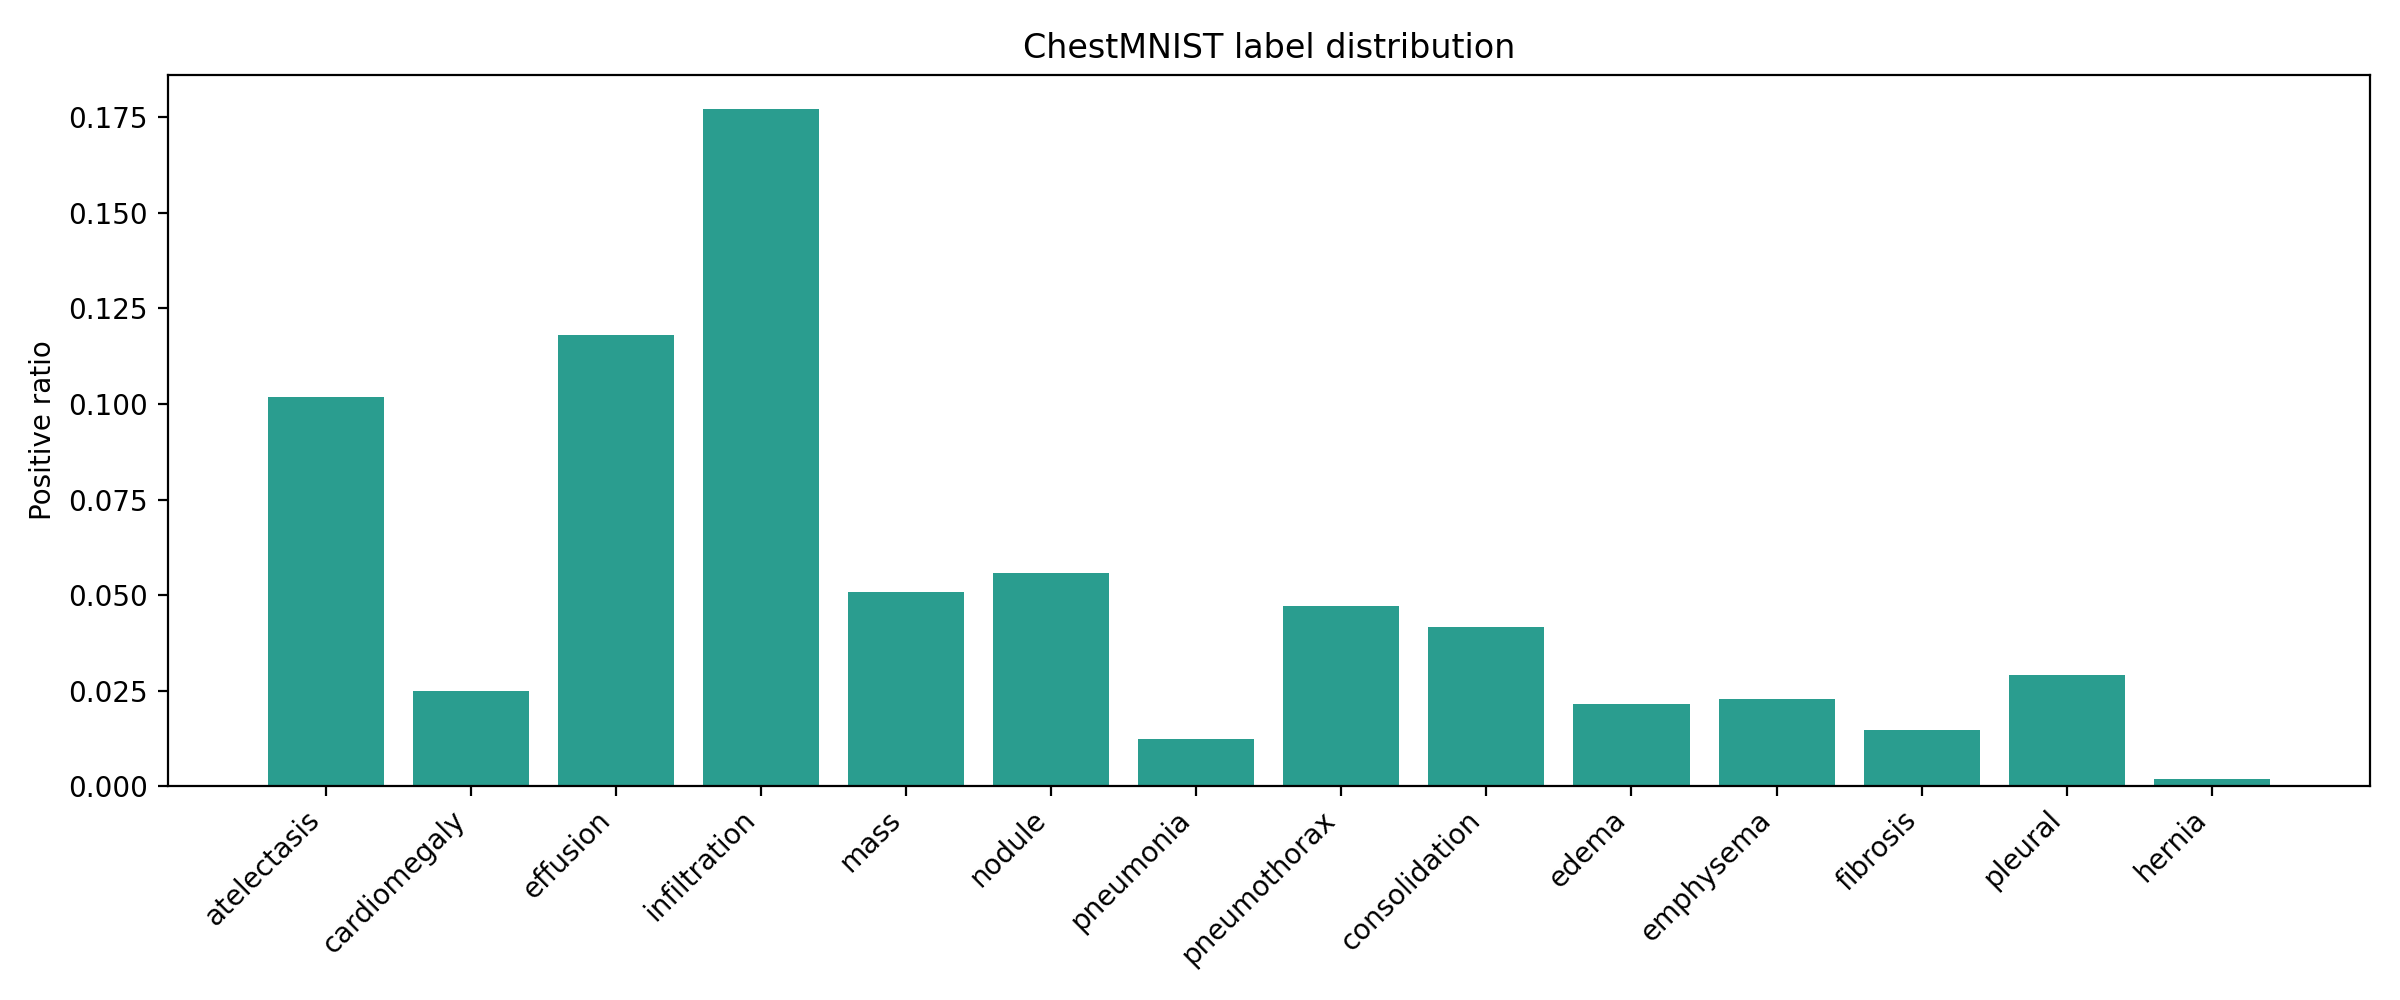
\includegraphics[width=0.82\textwidth]{../artifacts/eda/class_distribution.png}
    \caption{Distribution des classes positives dans le split d'entra\^\i nement ChestMNIST.}
\end{figure}

\begin{figure}[H]
    \centering
    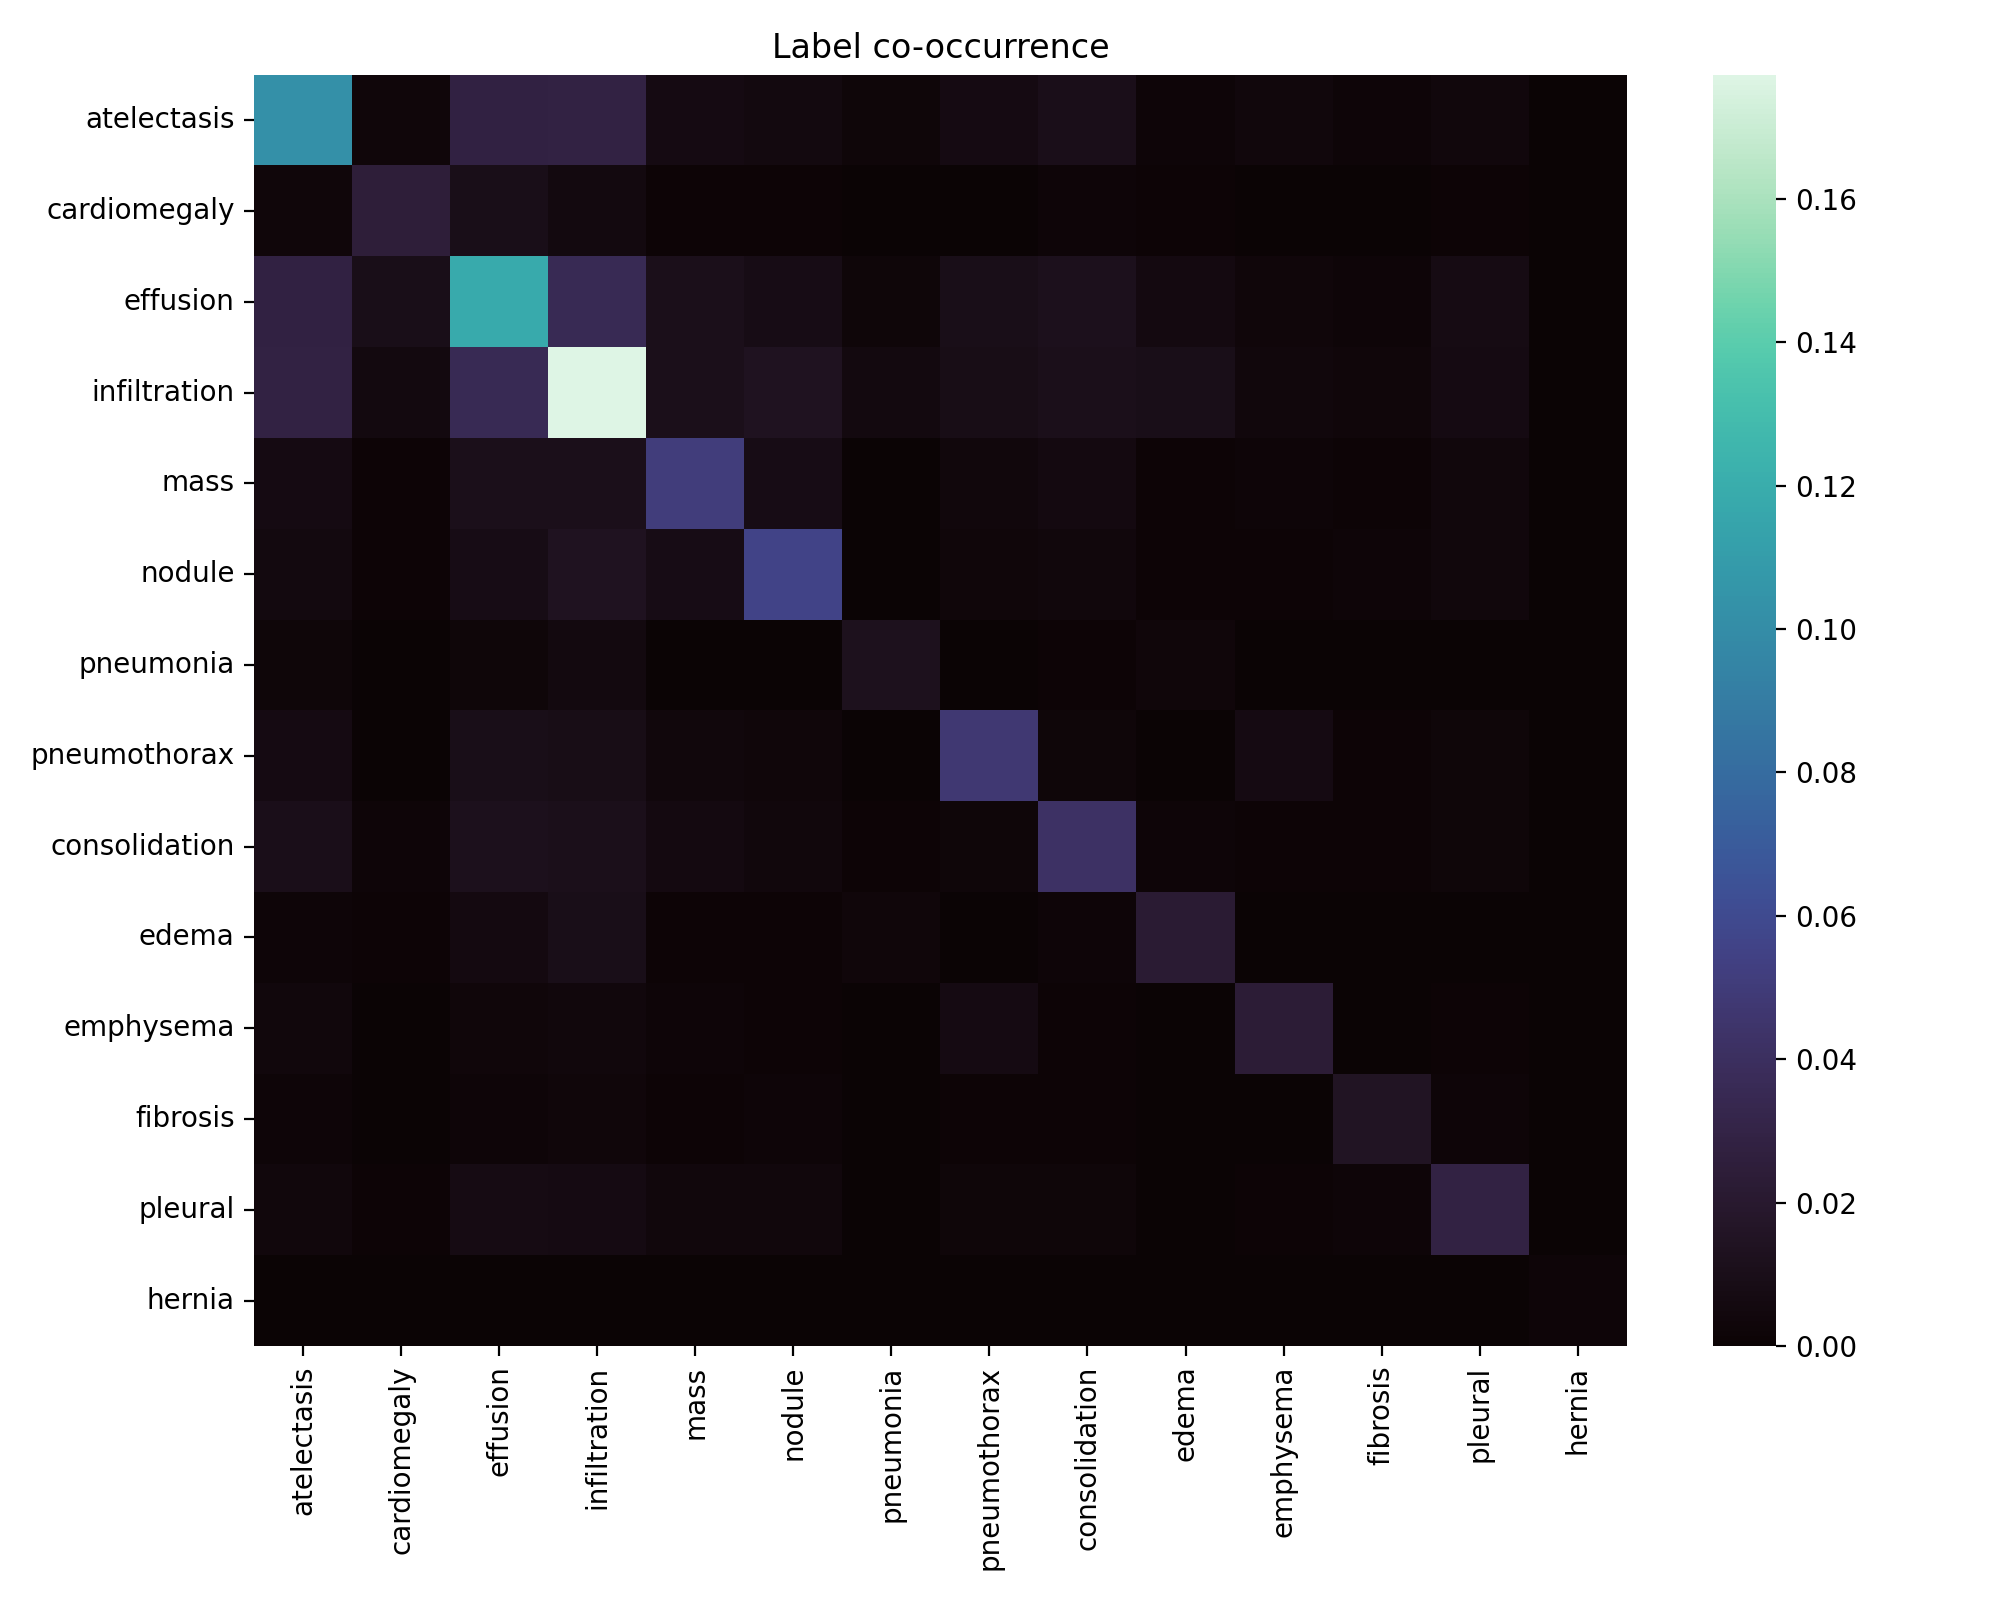
\includegraphics[width=0.82\textwidth]{../artifacts/eda/label_cooccurrence.png}
    \caption{Co-occurrences de labels dans ChestMNIST.}
\end{figure}

\begin{figure}[H]
    \centering
    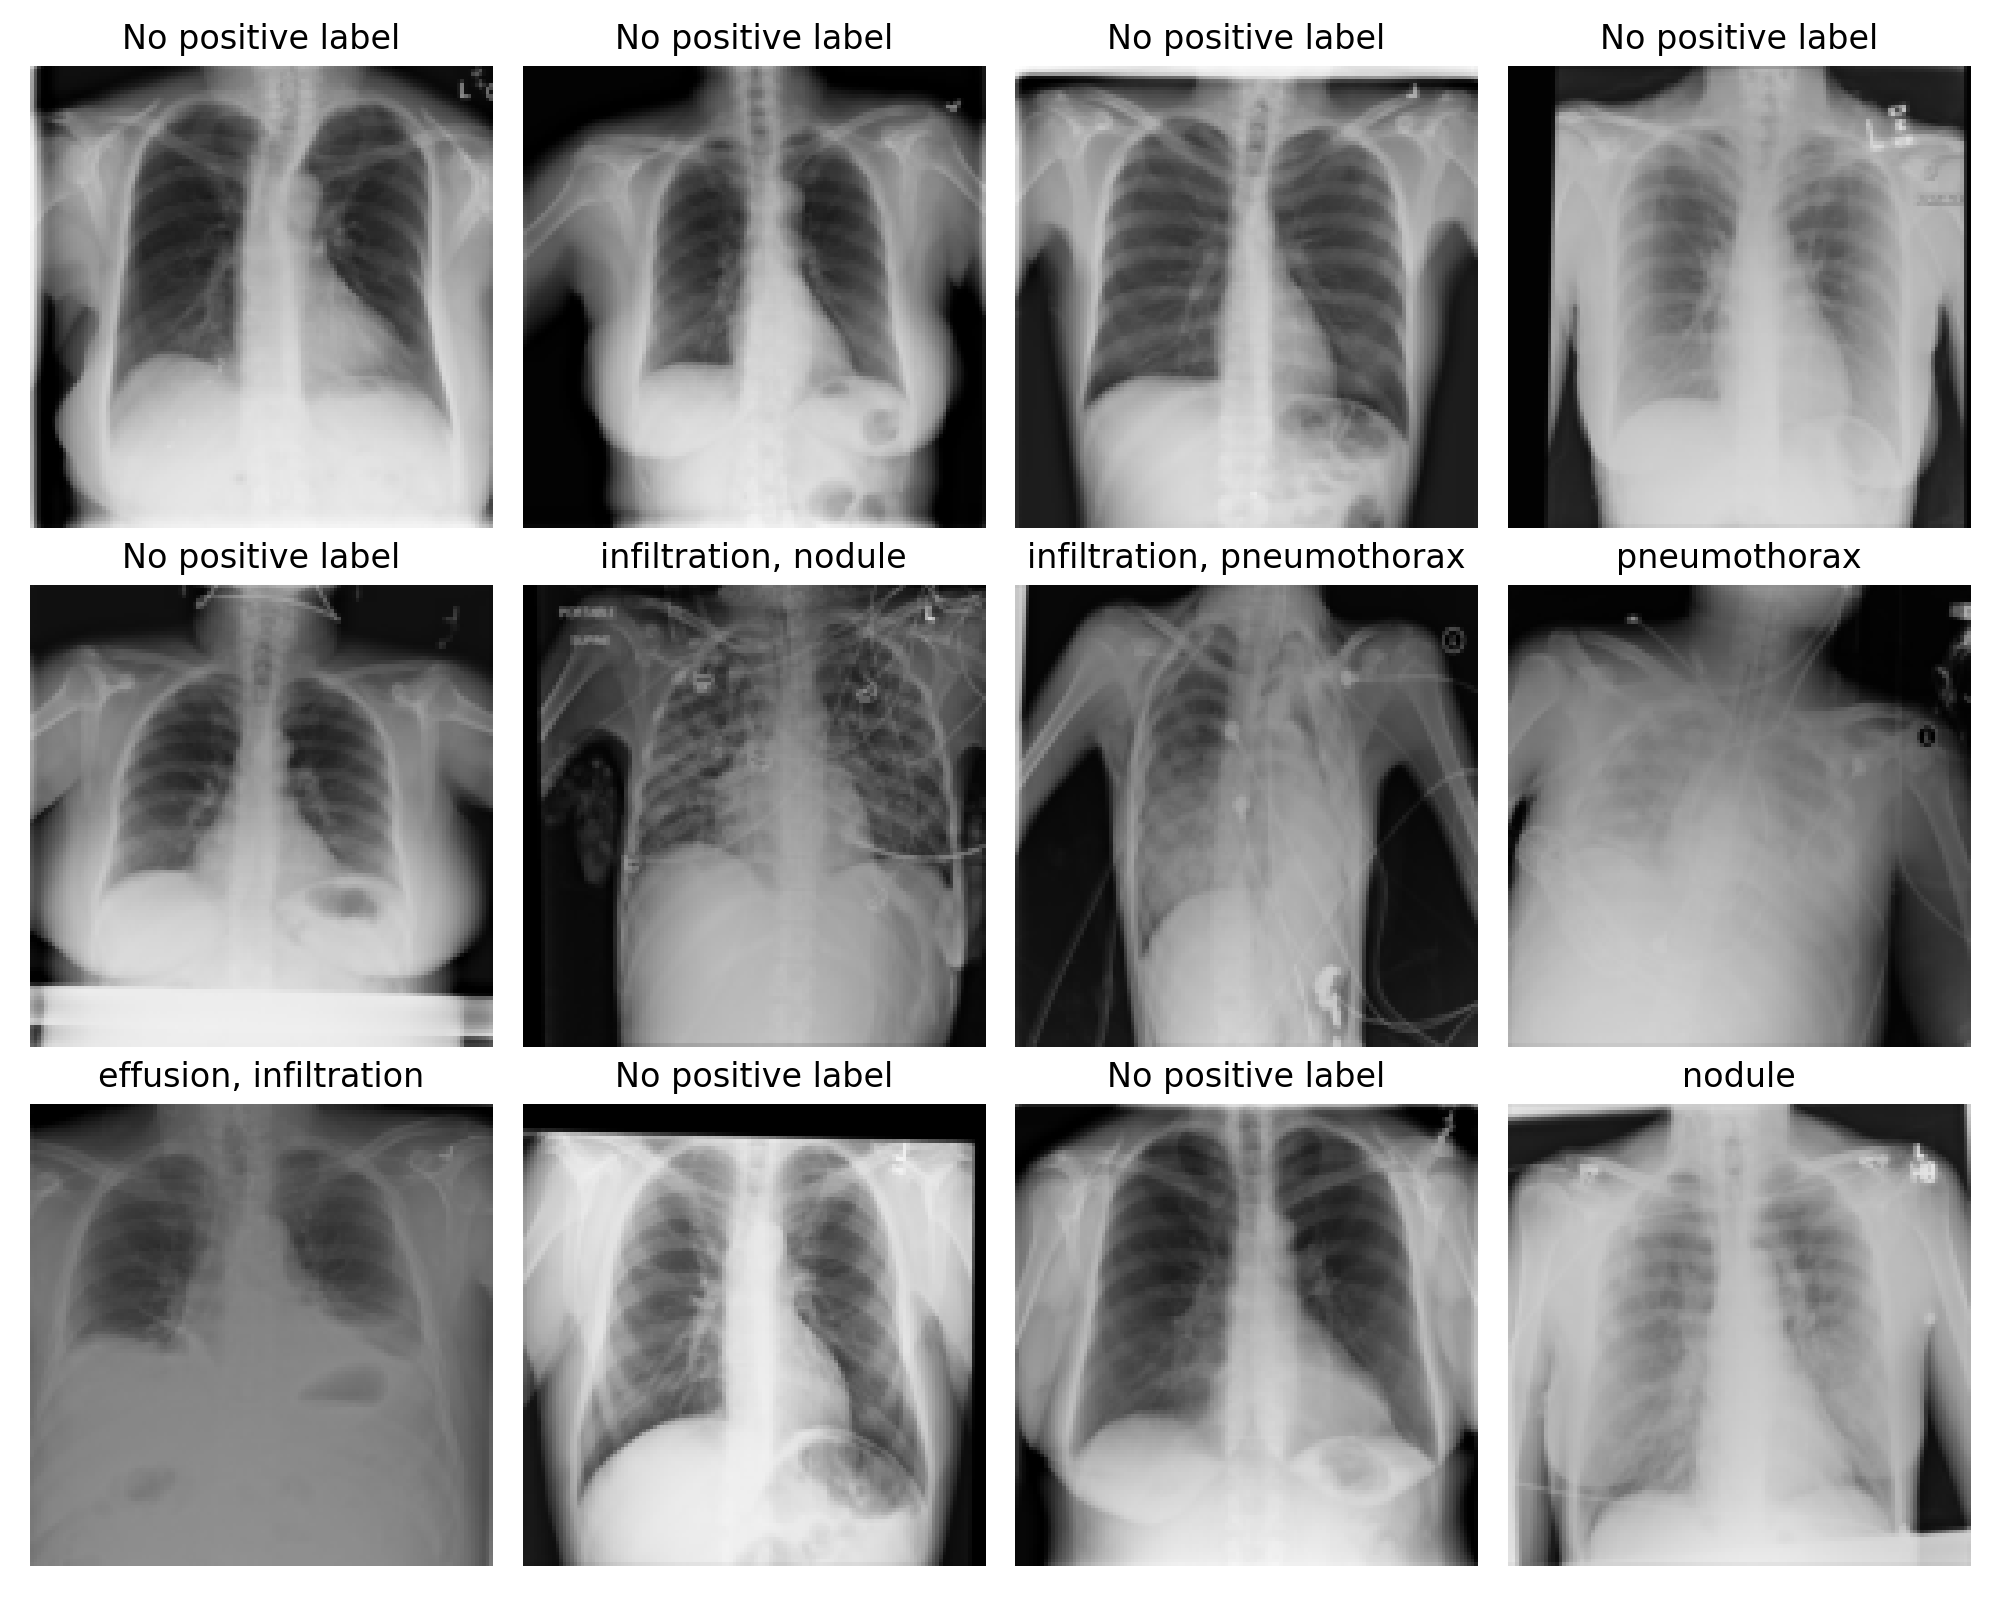
\includegraphics[width=0.82\textwidth]{../artifacts/eda/sample_images.png}
    \caption{Exemples de radiographies du split d'entra\^\i nement.}
\end{figure}

L'analyse exploratoire montre d'abord un fort d\'es\'equilibre. Dans le split d'entra\^\i nement, les pathologies les plus fr\'equentes sont \texttt{infiltration} (17.73\%), \texttt{effusion} (11.80\%) et \texttt{atelectasis} (10.19\%). \`A l'inverse, \texttt{hernia} (0.18\%), \texttt{pneumonia} (1.25\%) et \texttt{fibrosis} (1.48\%) sont rares. Environ 54.0\% des images du train ne portent aucun label positif, ce qui est particuli\`erement utile pour l'entra\^\i nement de l'autoencodeur sur des cas suppos\'es normaux.

Les co-occurrences les plus fortes concernent \texttt{effusion} + \texttt{infiltration}, \texttt{atelectasis} + \texttt{infiltration} et \texttt{atelectasis} + \texttt{effusion}. Ce point confirme que l'on est bien dans un contexte multi-label o\`u plusieurs atteintes peuvent \^etre pr\'esentes simultan\'ement.

Du c\^ot\'e textuel, IU X-Ray pr\'esente des comptes-rendus courts \`a moyens, avec une moyenne d'environ 31 tokens, une m\'ediane \`a 29 et un 90\ieme percentile \`a 50. Les labels d\'eriv\'es y sont eux aussi d\'es\'equilibr\'es: \texttt{effusion} et \texttt{pneumothorax} sont fr\'equents, alors que \texttt{hernia} et \texttt{edema} sont peu repr\'esent\'es.

\begin{table}[H]
    \centering
    \caption{Distribution des labels dans le split d'entra\^\i nement ChestMNIST.}
    \small
    \begin{tabular}{p{3.2cm}c c p{4.5cm}}
        \toprule
        Label & Positifs & Ratio & Commentaire \\
        \midrule
        atelectasis & 7\,996 & 10.19\% & classe fr\'equente, souvent co-occurrente avec effusion et infiltration \\
        cardiomegaly & 1\,950 & 2.49\% & support limit\'e mais cliniquement important \\
        effusion & 9\,261 & 11.80\% & l'une des pathologies les plus stables du corpus \\
        infiltration & 13\,914 & 17.73\% & classe la plus fr\'equente du jeu d'entra\^\i nement \\
        mass & 3\,988 & 5.08\% & interm\'ediaire, potentiellement h\'et\'erog\`ene \\
        nodule & 4\,375 & 5.58\% & classe sensible \`a la r\'esolution et au bruit \\
        pneumonia & 978 & 1.25\% & rare, donc difficile en termes de rappel \\
        pneumothorax & 3\,705 & 4.72\% & cliniquement pertinent pour le tri \\
        consolidation & 3\,263 & 4.16\% & fr\'equence moyenne \\
        edema & 1\,690 & 2.15\% & faible support, mais souvent discriminable \\
        emphysema & 1\,799 & 2.29\% & classe peu fr\'equente \\
        fibrosis & 1\,158 & 1.48\% & rare et potentiellement difficile \\
        pleural & 2\,279 & 2.90\% & support limit\'e \\
        hernia & 144 & 0.18\% & extr\^emement rare \\
        \bottomrule
    \end{tabular}
\end{table}

\subsection{Lecture qualitative de l'EDA}
L'EDA confirme que le probl\`eme n'est pas seulement un probl\`eme de reconnaissance visuelle. Il s'agit aussi d'un probl\`eme de calibration statistique. Dans un jeu fortement d\'es\'equilibr\'e, un mod\`ele peut apprendre \`a bien ranger les exemples par ordre de risque sans pour autant bien d\'etecter les classes rares au seuil de d\'ecision standard. C'est exactement la raison pour laquelle le rapport privil\'egie le ROC-AUC et l'Average Precision \`a l'accuracy brute.

Les exemples visuels r\'ev\`elent par ailleurs que plusieurs clich\'es sont peu contrast\'es, tr\`es homog\`enes ou marqu\'es par des diff\'erences d'acquisition. Ce constat justifie le choix d'augmentations l\'eg\`eres mais non agressives. Une augmentation trop forte pourrait artificiellement d\'egrader des motifs thoraciques d\'ej\`a fins dans les versions redimensionn\'ees du benchmark.

Les co-occurrences les plus fortes ne doivent pas \^etre interpr\'et\'ees comme des relations causales. Elles signalent plut\^ot que certains tableaux radiologiques ou certaines conventions d'annotation apparaissent ensemble plus souvent. D'un point de vue mod\'elisation, cela signifie qu'un classifieur multi-label peut exploiter des corr\'elations utiles, mais aussi qu'il risque d'apprendre des raccourcis entre classes au lieu de rep\'erer chaque signe visuel de mani\`ere ind\'ependante.

\subsection{Premiers constats sur le texte radiologique}
Le texte d'IU X-Ray contient majoritairement des formulations courtes, standardis\'ees, avec une forte r\'ep\'etition lexicale autour des motifs radiologiques classiques. Cette propri\'et\'e simplifie la vectorisation par vocabulaire et GRU, mais elle augmente aussi le risque que certaines expressions deviennent presque directement pr\'edictives des labels d\'eriv\'es. Ce point sera discut\'e plus loin dans l'analyse critique, car il influence fortement l'interpr\'etation des performances du mod\`ele texte seul et du mod\`ele fusionn\'e.

Du c\^ot\'e NIH, le texte structur\'e \texttt{metadata\_text} n'est pas un vrai langage narratif. Il agit plut\^ot comme une modalit\'e tabulaire serialis\'ee sous forme de cha\^\i ne. Son int\'er\^et est donc diff\'erent: il ne sert pas \`a tester une compr\'ehension s\'emantique riche, mais \`a v\'erifier qu'un pipeline multimodal peut exploiter proprement des informations non visuelles disponibles au moment du tri.

\section{Pr\'eparation des donn\'ees}
\subsection{Pr\'etraitement des images}
Pour la classification supervis\'ee, les images ChestMNIST sont redimensionn\'ees \`a la taille attendue par chaque mod\`ele. Une normalisation de type ImageNet est utilis\'ee pour les mod\`eles RGB. Des augmentations l\'eg\`eres sont activ\'ees en entra\^\i nement: retournement horizontal al\'eatoire et rotation faible. Pour l'autoencodeur, la normalisation est d\'esactiv\'ee afin de conserver une reconstruction directement interpr\'etable dans l'espace image.

Ce choix de pr\'etraitement est volontairement pragmatique. Dans un projet acad\'emique, il est tentant de multiplier les transformations, les normalisations sp\'ecifiques et les recettes de \emph{data augmentation}. Ici, l'objectif a \'et\'e de conserver un pipeline sobre, explicable et compatible avec plusieurs familles de mod\`eles. Les transformations retenues servent donc surtout \`a homog\'en\'eiser les tailles d'entr\'ee, limiter le surapprentissage et conserver une coh\'erence entre entra\^\i nement, \'evaluation et d\'emonstrateur.

La normalisation ImageNet pour les entr\'ees RGB peut sembler discutable dans un contexte m\'edical. Elle a cependant deux avantages pratiques: elle est directement compatible avec les backbones torchvision pr\'e-entra\^\i n\'es et elle stabilise les statistiques d'entr\'ee pour les branches convolutionnelles. Pour l'autoencodeur, cette normalisation aurait compliqu\'e l'interpr\'etation de la reconstruction. C'est pourquoi la branche anomalie conserve des images non normalis\'ees au sens ImageNet.

\subsection{Pr\'eparation des labels}
La t\^ache supervis\'ee est multi-label. Chaque sortie est donc trait\'ee par une perte \texttt{BCEWithLogitsLoss}. Afin de compenser partiellement le d\'es\'equilibre, des \texttt{pos\_weight} sont calcul\'es sur le train et int\'egr\'es \`a la fonction de perte lorsque la configuration l'autorise.

Pour l'anomalie, une cible binaire est d\'efinie par la pr\'esence d'au moins une pathologie positive. Les images normales du split train servent \`a apprendre la distribution de reconstruction, tandis que validation et test contiennent \`a la fois des cas normaux et anormaux.

Cette construction est importante, car elle s\'epare clairement l'objectif de reconstruction de l'objectif de classification. L'autoencodeur n'apprend pas \`a discriminer explicitement les maladies. Il apprend \`a reconstruire des exemples suppos\'es normaux. Le score d'anomalie d\'ecoule ensuite d'une d\'eviation par rapport \`a cette distribution. Il s'agit donc d'un usage \emph{indirect} des labels, limit\'e \`a la d\'efinition de la normalit\'e pendant la constitution du train.

\subsection{Pr\'eparation du texte}
Le texte multimodal est tokenis\'e par une r\`egle simple \`a base d'expressions r\'eguli\`eres, puis converti en indices via un vocabulaire construit exclusivement sur le split d'entra\^\i nement. Les s\'equences sont tronqu\'ees/padd\'ees \`a une longueur maximale de 128 tokens, avec une taille de vocabulaire plafonn\'ee \`a 5\,000 mots. Ce choix reste volontairement simple et reproductible.

Le recours \`a une tokenisation simple a \'et\'e pr\'ef\'er\'e \`a un tokenizer biom\'edical lourd pour trois raisons. D'abord, cela rend le pipeline totalement autonome et facilement ex\'ecutable hors ligne. Ensuite, cela simplifie fortement la sauvegarde et le rechargement dans l'application Streamlit. Enfin, dans un contexte de comptes-rendus relativement courts et fortement standardis\'es, une mod\'elisation lexicale simple constitue un point de d\'epart raisonnable avant d'envisager des encodeurs plus co\^uteux.

\subsection{Strat\'egie anti-fuite et reproductibilit\'e}
Le pipeline respecte plusieurs garde-fous:
\begin{itemize}
    \item splits officiels \texttt{train/val/test} pour ChestMNIST;
    \item split au niveau patient pour la variante NIH;
    \item vocabulaire textuel construit sur le train uniquement;
    \item calibrage du seuil d'anomalie sur la validation normale uniquement;
    \item seed fixe \texttt{42} avec configuration d\'eterministe PyTorch/CUDA;
    \item sauvegarde syst\'ematique du meilleur checkpoint de validation.
\end{itemize}

L'anti-fuite m\'erite une attention particuli\`ere dans un projet m\'edical. Une fuite ne provient pas seulement d'une mauvaise s\'eparation train/test. Elle peut aussi appara\^\i tre lorsqu'un vocabulaire textuel est construit sur l'ensemble du corpus, lorsqu'une calibration de seuil utilise des donn\'ees de test, ou lorsqu'un m\^eme patient peut se retrouver dans plusieurs splits. Les scripts du projet ont donc \'et\'e structur\'es pour que chaque \'etape de pr\'eparation soit index\'ee sur le split courant et ne regarde pas au-del\`a de ce qui lui est permis.

\subsection{Gestion du d\'es\'equilibre}
Le d\'es\'equilibre des labels thoraciques est un probl\`eme central du projet. Les classes les plus rares auraient \'et\'e rapidement \'ecras\'ees par les classes fr\'equentes si la perte n'avait pas \'et\'e pond\'er\'ee. La solution retenue consiste \`a calculer un \texttt{pos\_weight} par classe \`a partir du split d'entra\^\i nement. Ce choix n'annule pas compl\`etement le d\'es\'equilibre, mais il oblige l'optimisation \`a ne pas ignorer les classes rares.

Ce choix est plus sobre qu'une strat\'egie de sur-\emph{sampling} ou qu'une perte focalis\'ee. Il pr\'esente l'avantage de rester facile \`a tracer, \`a expliquer et \`a reproduire. Il s'accorde aussi avec l'objectif du projet, qui est de montrer un pipeline rigoureux avant de chercher des optimisations de pointe.

\subsection{Synth\`ese des pipelines de pr\'eparation}
\begin{table}[H]
    \centering
    \caption{Synth\`ese des pr\'etraitements appliqu\'es selon la composante du projet.}
    \small
    \begin{tabular}{p{3cm}p{2.4cm}p{3.1cm}p{2.4cm}p{3.3cm}}
        \toprule
        Composante & Taille image & Normalisation & Augmentation & Particularit\'e \\
        \midrule
        Supervision SimpleCNN & 128 & ImageNet & flip horizontal + rotation & apprentissage depuis z\'ero \\
        Supervision ResNet18 transfer & 224 & ImageNet & flip horizontal + rotation & transfer learning backbone gel\'e \\
        Supervision ResNet18 FT partiel & 224 & ImageNet & flip horizontal + rotation & \texttt{layer4 + fc} d\'egel\'es \\
        Supervision TinyViT & 128 & ImageNet & flip horizontal + rotation & patches + encodeur Transformer compact \\
        Autoencodeur & 64 & aucune & l\'eg\`ere augmentation train & reconstruction en espace image \\
        Multimodal IU X-Ray & 128 & ImageNet & flip horizontal train & texte vectoris\'e, max length 128 \\
        \bottomrule
    \end{tabular}
\end{table}

\subsection{Methodologie de conduite de projet}
Au-del\`a de la m\'ethodologie d'apprentissage, l'organisation du travail a suivi une logique de pilotage par \textbf{tableau Kanban}. Cette approche a \'et\'e retenue pour structurer le projet en t\^aches courtes, visibles et r\'eparties entre les grandes briques impos\'ees par le sujet: donn\'ees, EDA, mod\'elisation supervis\'ee, anomalie, multimodalit\'e, tracking MLflow, application et rapport.

Le tableau Kanban a permis de distinguer explicitement plusieurs \'etats de travail, par exemple:
\begin{itemize}
    \item \emph{\`a faire} pour les t\^aches identifi\'ees mais non commenc\'ees;
    \item \emph{en cours} pour les composants en d\'eveloppement ou en entra\^\i nement;
    \item \emph{\`a valider} pour les t\^aches techniquement termin\'ees mais encore en attente de v\'erification;
    \item \emph{termin\'e} pour les livrables stabilis\'es et int\'egr\'es au d\'ep\^ot.
\end{itemize}

Cette m\'ethode pr\'esente un int\'er\^et particulier dans un projet de deep learning, car le temps de travail n'est pas uniquement du temps de codage. Une partie importante du projet est consomm\'ee par le t\'el\'echargement et la pr\'eparation des jeux de donn\'ees, les essais de configurations, les temps d'entra\^\i nement, l'analyse des artefacts MLflow et la r\'edaction du rapport. Le tableau Kanban a donc servi \`a visualiser les d\'ependances entre t\^aches et \`a maintenir une progression coh\'erente entre exp\'erimentation, validation technique et production des livrables.

Dans le rapport, ce point m\'ethodologique est important car il explique la mani\`ere dont le projet a \'et\'e conduit: non pas comme une suite informelle d'essais, mais comme un encha\^\i nement organis\'e de t\^aches pilot\'ees, prioris\'ees et valid\'ees au fur et \`a mesure de l'avancement.

\subsection{Demarche methodologique generale}
La m\'ethodologie suivie dans le projet peut \^etre r\'esum\'ee comme une d\'emarche it\'erative et reproductible articul\'ee autour de six \'etapes. La premi\`ere a consist\'e \`a cadrer le sujet et \`a le d\'ecouper en briques fonctionnelles coh\'erentes: classification supervis\'ee, anomalie, multimodalit\'e, tracking exp\'erimental, application et rapport. Cette phase de cadrage a \'et\'e directement reli\'ee au tableau Kanban, qui a servi de support de planification et de priorisation.

La deuxi\`eme \'etape a concern\'e l'acquisition et la structuration des donn\'ees. Elle a consist\'e \`a s\'electionner `ChestMNIST` comme base principale pour la partie image, `IU X-Ray / OpenI` pour la composante \emph{image + texte}, puis `NIH Chest X-rays` comme variante compl\'ementaire. Les scripts d'import ont \'et\'e con\c{c}us pour produire des formats exploitables directement par les loaders PyTorch du projet, avec une s\'eparation claire entre fichiers bruts, CSV pr\'epar\'es et r\'esum\'es d'import.

La troisi\`eme \'etape a \'et\'e l'analyse exploratoire. Son objectif n'\'etait pas seulement descriptif, mais d\'ecisionnel. L'EDA a permis d'identifier le d\'es\'equilibre des classes, de visualiser les co-occurrences de labels, d'observer le type d'images disponibles et d'\'evaluer la structure du texte radiologique. Ces observations ont ensuite guid\'e les choix de pr\'etraitement, de m\'etriques et de pond\'eration des classes.

La quatri\`eme \'etape a \'et\'e la mise en place des protocoles d'entra\^\i nement. Pour la supervision, l'objectif a \'et\'e de comparer trois familles de mod\`eles correspondant explicitement aux exigences du sujet. Pour la d\'etection d'anomalies, la m\'ethodologie a repos\'e sur l'apprentissage d'une distribution normale puis sur la calibration d'un seuil de reconstruction. Pour la multimodalit\'e, la d\'emarche a consist\'e \`a comparer des baselines unimodales \`a un mod\`ele de fusion, afin d'isoler l'apport r\'eel de la seconde modalit\'e.

La cinqui\`eme \'etape a port\'e sur l'\'evaluation et la tra\c{c}abilit\'e. Les exp\'eriences ont \'et\'e enregistr\'ees dans MLflow avec leurs hyperparam\`etres, leurs m\'etriques, leurs artefacts visuels et leurs checkpoints. Cette phase a permis de conserver une continuit\'e entre entra\^\i nement, comparaison de runs, s\'election des mod\`eles et int\'egration dans l'application.

Enfin, la sixi\`eme \'etape a concern\'e l'industrialisation acad\'emique du projet, c'est-\`a-dire la production d'un d\'emonstrateur exploitable et d'un rapport argument\'e. La logique suivie a donc \'et\'e la suivante: partir des donn\'ees, construire des pipelines reproductibles, comparer les approches, tracer les r\'esultats, puis transformer ces r\'esultats en livrables coh\'erents et pr\'esentables.

\subsection{Outils et environnement exp\'erimental}
Le projet repose principalement sur Python 3.11, PyTorch 2.11, Torchvision, MedMNIST, pandas, scikit-learn, MLflow et Streamlit. L'ex\'ecution finale a \'et\'e relanc\'ee sur une machine Windows 11 dot\'ee d'un processeur Intel Core i7-10750H, de 16 Go de RAM et d'un GPU NVIDIA GeForce RTX 2070 Max-Q avec CUDA 12.8.

Le mat\'eriel utilis\'e fait partie int\'egrante de la m\'ethodologie du projet, car il conditionne directement les r\'esolutions retenues, la taille des batches, le nombre d'\'epoques, le choix d'un \emph{TinyViT} compact plut\^ot qu'un Transformer plus lourd, ainsi que la dur\'ee totale d'ex\'ecution de la pipeline finale. L'ensemble des entra\^\i nements finaux, du suivi MLflow, des tests applicatifs et de la compilation du rapport a \'et\'e r\'ealis\'e dans cet environnement local.

\begin{table}[H]
    \centering
    \caption{Configuration mat\'erielle et logicielle utilis\'ee pour le projet.}
    \begin{tabular}{p{5cm}p{8cm}}
        \toprule
        El\'ement & Valeur \\
        \midrule
        OS & Windows 11 Famille (build 10.0.26200) \\
        CPU & Intel Core i7-10750H, 6 coeurs / 12 threads \\
        RAM & 16 Go \\
        GPU & NVIDIA GeForce RTX 2070 with Max-Q Design \\
        VRAM & environ 8 Go \\
        Python & 3.11.9 \\
        PyTorch & 2.11.0+cu128 \\
        Torchvision & 0.26.0+cu128 \\
        Framework d'app & Streamlit 1.53.1 \\
        Tracking & MLflow 3.10.1 \\
        \bottomrule
    \end{tabular}
\end{table}

\subsection{Contraintes de calcul et choix de compromis}
Le mat\'eriel disponible a influenc\'e plusieurs choix d'architecture et d'hyperparam\`etres. Un GPU de type RTX 2070 Max-Q permet de lancer l'ensemble du projet, mais il ne rend pas pour autant tous les choix calculatoires gratuits. En particulier, un ViT standard pr\'e-entra\^\i n\'e \`a grande r\'esolution aurait impos\'e un co\^ut m\'emoire et temporel beaucoup plus important. C'est l'une des raisons qui ont conduit \`a l'introduction d'un \emph{TinyViT} maison, plus modeste mais plus compatible avec un rendu de projet complet.

De m\^eme, le nombre d'\'epoques, les tailles de batch, la r\'esolution des images et l'usage soit du gel du backbone soit d'un d\'egel partiel dans ResNet18 ont \'et\'e pens\'es comme des compromis entre qualit\'e d'apprentissage, dur\'ee d'ex\'ecution et stabilit\'e globale. Dans un cadre industriel, ces compromis seraient probablement rediscut\'es sur des serveurs multi-GPU ou sur des benchmarks plus lourds. Dans un cadre acad\'emique, ils permettent de conserver un pipeline final r\'ealiste et ex\'ecutable de bout en bout.

\section{Mod\'elisation supervis\'ee}
Trois familles de mod\`eles sont compar\'ees pour la partie supervis\'ee.

Le choix de ces trois familles r\'epond directement \`a la consigne du sujet, mais il suit aussi une logique exp\'erimentale. Le \textbf{SimpleCNN} sert de baseline contr\^ol\'ee. \textbf{ResNet18} sert de point de comparaison en transfer learning avec un backbone largement standardis\'e, d'abord en mode backbone gel\'e puis en fine-tuning partiel plus ambitieux. \textbf{TinyViT} sert enfin \`a repr\'esenter le paradigme Transformer sans rendre le co\^ut d'entra\^\i nement prohibitif. Ensemble, ces trois familles permettent de discuter non seulement les performances, mais aussi la sensibilit\'e au calcul, la facilit\'e de convergence et la coh\'erence avec les contraintes du projet.

\subsection{CNN simple entra\^\i n\'e depuis z\'ero}
Le premier mod\`ele est un CNN compact con\c{c}u pour l'apprentissage \`a partir de z\'ero. Il empile quatre blocs convolution + batch normalization + ReLU, suivis d'un \emph{adaptive average pooling} et d'une couche lin\'eaire finale. Cette architecture sert de base de comparaison franche: elle est plus l\'eg\`ere, plus rapide \`a entra\^\i ner et plus facile \`a interpr\'eter qu'un backbone pr\'e-entra\^\i n\'e.

Ce mod\`ele est particuli\`erement int\'eressant pour un projet p\'edagogique, car il permet de mesurer ce que le pipeline apprend \emph{vraiment} sans h\'eritage fort issu d'un pr\'e-entra\^\i nement externe. Si les performances sont d\'ej\`a raisonnables, cela signifie que la cha\^\i ne de donn\'ees, la fonction de perte, les m\'etriques et la gestion des splits sont saines. En ce sens, le CNN simple joue aussi le r\^ole de garde-fou exp\'erimental.

\subsection{CNN pr\'e-entra\^\i n\'e avec transfer learning}
Le deuxi\`eme mod\`ele est un ResNet18 \cite{he2016resnet} pr\'e-entra\^\i n\'e sur ImageNet. Deux r\'egimes ont \'et\'e \'evalu\'es dans le projet. Le premier conserve le backbone gel\'e et n'optimise que la t\^ete de classification, ce qui fournit une base de transfer learning rapide et stable. Le second d\'eg\`ele seulement \texttt{layer4} et \texttt{fc}, avec un learning rate plus faible pour le backbone que pour la t\^ete. Cette seconde variante, ex\'ecut\'ee en r\'esolution 224, constitue finalement le meilleur run supervis\'e du projet.

Le gel complet du backbone r\'eduit le nombre de param\`etres effectivement optimis\'es, acc\'el\`ere l'entra\^\i nement et diminue le risque d'instabilit\'e dans un contexte o\`u la taille d'image et la taille de lot restent mod\'er\'ees. En contrepartie, il limite l'adaptation fine du mod\`ele au domaine radiologique. Le d\'egel partiel de \texttt{layer4 + fc} offre un compromis plus convaincant: l'essentiel du backbone reste stable, mais les derni\`eres repr\'esentations peuvent mieux s'aligner sur la radiologie thoracique sans exploser le co\^ut d'entra\^\i nement.

\subsection{Vision Transformer compact}
Le troisi\`eme mod\`ele est un petit transformer visuel inspir\'e de ViT \cite{dosovitskiy2021vit}. Il ne s'agit pas d'un ViT industriel pr\'e-entra\^\i n\'e, mais d'une impl\'ementation compacte adapt\'ee aux ressources disponibles: extraction de patches par convolution, ajout d'un jeton \texttt{cls}, embeddings positionnels appris, encodeur Transformer puis t\^ete lin\'eaire. L'int\'er\^et de cette architecture est de couvrir explicitement la famille Transformer demand\'ee par le sujet.

Cette architecture ne doit pas \^etre lue comme une tentative de battre tous les mod\`eles convolutionnels sur ce benchmark. Elle est plut\^ot con\c{c}ue comme une exploration du paradigme Transformer dans un cadre mat\'eriel raisonnable. Le rapport met donc autant l'accent sur la justification du choix que sur le chiffre brut final.

\subsection{Choix d'optimisation}
Les entra\^\i nements supervis\'es utilisent AdamW, un scheduler cosinus, un \texttt{early stopping} sur la validation et une BCE multi-label pond\'er\'ee. Les tailles d'images et de batch diff\`erent selon les mod\`eles afin de conserver un co\^ut calculatoire raisonnable.

Le protocole de comparaison cherche \`a \^etre homog\`ene sans \^etre artificiellement identique. Il aurait \'et\'e possible d'imposer la m\^eme taille d'image et le m\^eme batch \`a tous les mod\`eles, mais cela aurait p\'enalis\'e inutilement certaines architectures. Le parti pris retenu consiste donc \`a conserver une m\^eme philosophie d'optimisation tout en adaptant la r\'esolution et le batch size \`a la famille de mod\`ele.

\begin{table}[H]
    \centering
    \caption{Configurations principales des mod\`eles supervis\'es.}
    \small
    \begin{tabular}{p{3.1cm}c c c c c}
        \toprule
        Mod\`ele & Taille image & Batch size & Epoques max & Learning rate & Particularit\'e \\
        \midrule
        SimpleCNN & 128 & 64 & 10 & 1e-3 & apprentissage depuis z\'ero \\
        ResNet18 transfer & 224 & 32 & 5 & 3e-4 & backbone pr\'e-entra\^\i n\'e gel\'e \\
        ResNet18 partial FT 224 & 224 & 24 & 12 & 2e-4 / 2e-5 & \texttt{layer4 + fc}, learning rates diff\'erenci\'es \\
        TinyViT & 128 & 32 & 6 & 3e-4 & encodeur Transformer compact \\
        \bottomrule
    \end{tabular}
\end{table}

\subsection{Crit\`eres de comparaison}
Les trois familles de mod\`eles ne sont pas compar\'ees uniquement sur la qualit\'e du ROC-AUC final. Quatre dimensions sont consid\'er\'ees:
\begin{itemize}
    \item la qualit\'e de classement multi-label sur le test;
    \item la stabilit\'e de la validation au cours des \'epoques;
    \item le rapport entre co\^ut de calcul et gain obtenu;
    \item la facilit\'e de r\'eutilisation dans le d\'emonstrateur applicatif.
\end{itemize}

Ce dernier point est important. Un mod\`ele excellent mais trop lourd \`a charger ou trop lent \`a inf\'erer dans l'application perd une partie de son int\'er\^et dans un projet orient\'e d\'emonstration. La dimension syst\`eme oblige donc \`a d\'epasser la seule logique ``leaderboard''.

\section{D\'etection d'anomalies par AE / VAE}
La brique d'anomalie repose sur un autoencodeur convolutionnel simple. L'encodeur applique trois convolutions strid\'ees successives et compresse l'image vers un espace latent de 128 canaux. Le d\'ecodeur reconstruit ensuite l'image par convolutions transpos\'ees.

La perte retenue est une \texttt{L1Loss} entre image d'origine et reconstruction. Le score d'anomalie est la moyenne des erreurs absolues de reconstruction par pixel. L'intuition est directe: si le mod\`ele a surtout vu des cas normaux, il doit moins bien reconstruire les cas pathologiques, atypiques ou hors distribution.

Le seuil de d\'ecision est calibr\'e sur la validation \`a partir du 95\ieme percentile des scores des cas normaux. Ce choix simple a l'avantage d'\^etre tra\c{c}able, facilement reproductible et compatible avec une interface de d\'emonstration.

\subsection{Pourquoi un autoencodeur dans ce projet}
La brique d'anomalie a un r\^ole diff\'erent de la classification supervis\'ee. Elle n'a pas vocation \`a dire \emph{quelle} pathologie est pr\'esente, mais \`a signaler qu'une image s'\'ecarte de ce que le mod\`ele consid\`ere comme habituel. Dans un sc\'enario de tri, cette information compl\'emente utilement les probabilit\'es supervis\'ees. Une image peut obtenir une pr\'ediction mod\'er\'ee sur plusieurs classes tout en pr\'esentant un score d'anomalie \'elev\'e, ce qui peut justifier une relecture prioritaire.

Le choix d'un autoencodeur plut\^ot que d'un VAE est li\'e \`a la lisibilit\'e du projet. L'AE convolutionnel est plus direct \`a impl\'ementer, plus facile \`a expliquer dans un rapport de master ou d'ing\'enieur, et suffisamment expressif pour d\'emontrer le principe d'une d\'etection par reconstruction. Un VAE aurait ajout\'e une couche de complexit\'e probabiliste utile, mais non indispensable pour la preuve de concept vis\'ee ici.

\subsection{Protocole d'entra\^\i nement}
L'entr\'ee du mod\`ele est une radiographie redimensionn\'ee en 64\,$\times$\,64. Le train ne contient que des images sans label positif, de sorte que le mod\`ele apprenne prioritairement une distribution ``normale''. La validation et le test contiennent \`a la fois des cas normaux et anormaux, ce qui permet de mesurer la qualit\'e discriminante du score de reconstruction.

Le protocole suivi est le suivant:
\begin{itemize}
    \item apprentissage sur le split train normal uniquement;
    \item calcul des scores d'erreur absolue moyenne sur le split val;
    \item d\'efinition d'un seuil \`a partir du quantile 95\% des cas normaux de validation;
    \item application du m\^eme seuil au split test pour obtenir F1, pr\'ecision, rappel et accuracy;
    \item journalisation des reconstructions et de l'histogramme des scores dans MLflow.
\end{itemize}

Cette cha\^\i ne est simple, mais elle poss\`ede une vraie logique exp\'erimentale. Le seuil n'est pas choisi \emph{a posteriori} sur le test; il est calibr\'e avant toute \'evaluation finale. Cette distinction est essentielle pour maintenir une interpr\'etation correcte des r\'esultats.

\subsection{Interpr\'etation du score d'anomalie}
Le score calcul\'e ne mesure pas directement une distance clinique \`a une pathologie. Il mesure une difficult\'e de reconstruction dans l'espace image. Une erreur \'elev\'ee peut provenir d'une l\'esion, mais aussi d'un artefact d'acquisition, d'un cadrage inhabituel, d'un contraste atypique ou d'un motif anatomique peu fr\'equent dans les cas normaux du train. En pratique, cela veut dire qu'un score d'anomalie doit \^etre interpr\'et\'e comme un signal de vigilance, pas comme un diagnostic.

Cette propri\'et\'e est en r\'ealit\'e coh\'erente avec le cahier des charges du sujet. Le projet doit \emph{identifier des cas atypiques, ambigus, rares ou hors distribution}. La cat\'egorie vis\'ee est donc plus large que la maladie au sens strict. Un bon module d'anomalie peut avoir de la valeur m\^eme s'il ne distingue pas parfaitement toutes les pathologies.

\subsection{Points forts et limites}
L'approche par autoencodeur pr\'esente plusieurs avantages. Elle est simple, visuelle, explicable, et produit des artefacts d'analyse qualitatifs tr\`es utiles dans un rapport: grilles de reconstruction, histogrammes de scores, inspection des faux positifs et faux n\'egatifs. Elle est aussi ind\'ependante de la t\^ache de classification proprement dite, ce qui apporte une forme de redondance utile au syst\`eme.

Ses limites sont toutefois importantes. D'une part, la notion de normalit\'e apprise d\'epend fortement du train disponible. D'autre part, la reconstruction peut rester de bonne qualit\'e sur certains cas pathologiques r\'ep\'etitifs, et inversement se d\'egrader sur des variations non pathologiques. Enfin, l'\'evaluation binaire ``normal vs au moins un label positif'' simplifie fortement la r\'ealit\'e clinique. Cette brique doit donc \^etre comprise comme un module d'alerte exploratoire, pas comme un outil autonome de d\'ecision.

\section{Mod\'elisation multimodale image + compte-rendu}
\subsection{Repr\'esentation image}
La voie image multimodale utilise un petit encodeur convolutionnel produisant un embedding dense de taille 128. Cette branche est volontairement l\'eg\`ere afin que la comparaison \emph{image seule / texte seul / fusion} mette davantage en \'evidence l'apport de la modalit\'e textuelle que l'effet d'un backbone tr\`es profond.

L'int\'er\^et de cette simplicit\'e est aussi m\'ethodologique. Si la branche image \'etait trop puissante, la fusion pourrait ne presque rien apporter, simplement parce que l'image seule dominerait le probl\`eme. A l'inverse, une branche image trop faible rendrait la fusion artificiellement d\'ependante du texte. Le petit encodeur convolutionnel constitue donc un compromis raisonnable pour comparer les trois variantes de mani\`ere plus lisible.

\subsection{Repr\'esentation texte}
La voie texte repose sur une couche d'embedding, suivie d'un GRU bidirectionnel et d'un pooling masqu\'e par \texttt{attention\_mask}. Cette approche reste plus simple qu'un encodeur de type BERT, mais elle est parfaitement suffisante pour une preuve de concept reproductible.

Le GRU bidirectionnel pr\'esente plusieurs avantages dans ce contexte. Il capture l'ordre local des mots mieux qu'un simple sac de mots, reste plus l\'eger qu'un transformeur de langage, et se recharge facilement dans l'application. Sur des comptes-rendus courts, il peut suffire \`a repr\'esenter l'information s\'emantique essentielle sans faire exploser le temps d'entra\^\i nement.

\subsection{Strat\'egie de fusion}
La fusion retenue est une \textbf{fusion interm\'ediaire}: les repr\'esentations image et texte sont encod\'ees s\'epar\'ement, concat\'en\'ees, puis inject\'ees dans une petite t\^ete MLP. En entra\^\i nement, un \emph{modality dropout} peut annuler al\'eatoirement une partie de l'information image ou texte, afin de tester une forme minimale de robustesse \`a l'absence d'une modalit\'e.

Ce choix de fusion a \'et\'e retenu pour des raisons \`a la fois conceptuelles et pratiques. Une fusion pr\'ecoce aurait impos\'e d'harmoniser tr\`es t\^ot des donn\'ees de nature radicalement diff\'erente. Une fusion tardive, elle, aurait davantage rapproch\'e le probl\`eme d'un assemblage de scores. La fusion interm\'ediaire permet au contraire de laisser chaque modalit\'e construire une repr\'esentation adapt\'ee avant interaction, ce qui est bien align\'e avec un projet de preuve de concept.

\subsection{Organisation des exp\'eriences multimodales}
Trois runs distincts sont pr\'evus sur la branche IU X-Ray:
\begin{itemize}
    \item \texttt{image\_only}: l'image est la seule modalit\'e active;
    \item \texttt{text\_only}: seule la s\'equence textuelle est utilis\'ee;
    \item \texttt{fusion}: les deux repr\'esentations sont concat\'en\'ees avant pr\'ediction.
\end{itemize}

Cette structure est fondamentale pour l'interpr\'etation. Un score de fusion n'a de sens que s'il est compar\'e \`a des branches unimodales entra\^\i n\'ees dans un cadre coh\'erent. Sans ces baselines, il serait impossible de savoir si la multimodalit\'e aide vraiment ou si une seule modalit\'e portait d\'ej\`a presque toute l'information utile.

\subsection{Comparaisons pr\'evues}
Conform\'ement au sujet, trois variantes sont impl\'ement\'ees:
\begin{itemize}
    \item un mod\`ele \emph{image only};
    \item un mod\`ele \emph{text only};
    \item un mod\`ele \emph{fusion image + texte}.
\end{itemize}

Cette comparaison doit toutefois \^etre interpr\'et\'ee avec prudence sur IU X-Ray, car les labels sont extraits du compte-rendu. Si le texte domine trop fortement, cela peut traduire moins un gain multimodal qu'un raccourci s\'emantique li\'e au weak labeling.

\subsection{Robustesse \`a l'absence d'une modalit\'e}
Le code du projet inclut un test suppl\'ementaire sur le mod\`ele de fusion: l'\'evaluation avec texte d\'esactiv\'e et l'\'evaluation avec image d\'esactiv\'ee. Cette exp\'erience est int\'eressante \`a double titre. D'une part, elle renseigne sur la d\'ependance r\'eelle du mod\`ele \`a chaque modalit\'e. D'autre part, elle rapproche le pipeline d'un usage applicatif r\'ealiste dans lequel le texte peut \^etre absent, partiel ou de mauvaise qualit\'e.

Dans une lecture saine des r\'esultats, un mod\`ele de fusion n'est pas n\'ecessairement meilleur parce qu'il obtient le plus haut score absolu. Il peut aussi \^etre meilleur parce qu'il se d\'egrade plus gracieusement lorsqu'une modalit\'e manque, ou parce qu'il reste plus stable qu'une branche unimodale face \`a certains cas ambigus.

\subsection{Variante NIH et discussion m\'ethodologique}
La variante NIH n'est pas le coeur de la comparaison finale, mais elle est utile pour discuter un point souvent oubli\'e dans les projets multimodaux: en pratique, la ``modalit\'e texte'' n'est pas toujours un compte-rendu libre. Elle peut \^etre un ensemble de m\'etadonn\'ees patient, d'informations de contexte ou d'annotations semi-structur\'ees. Construire \texttt{metadata\_text} sous forme s\'equentielle permet de r\'eutiliser la m\^eme infrastructure de chargement, de vocabulaire et de mod\`ele texte sans cr\'eer un pipeline totalement s\'epar\'e.

Cette d\'ecision a un int\'er\^et p\'edagogique fort. Elle montre que la multimodalit\'e du projet n'est pas limit\'ee \`a un cas unique, mais qu'elle repose sur une abstraction logicielle suffisamment g\'en\'erale pour accepter plusieurs types de deuxi\`eme modalit\'e.

\section{\'Evaluation}
Dans un cadre multi-label et fortement d\'es\'equilibr\'e, l'accuracy seule est insuffisante. Les m\'etriques retenues dans le code sont:
\begin{itemize}
    \item ROC-AUC macro et micro;
    \item Average Precision macro et micro;
    \item F1 macro et micro;
    \item accuracy par sous-ensemble, utilis\'ee uniquement comme indicateur secondaire;
    \item analyse par classe \`a partir des courbes, barplots et matrices de confusion adapt\'ees.
\end{itemize}

\subsection{Pourquoi ces m\'etriques}
Le choix des m\'etriques n'est pas un d\'etail de pr\'esentation. Il conditionne la mani\`ere dont on juge un syst\`eme de tri. Le ROC-AUC \'evalue la capacit\'e du mod\`ele \`a classer les positifs avant les n\'egatifs, ind\'ependamment d'un seuil fixe. L'Average Precision est plus sensible au d\'es\'equilibre et donc particuli\`erement informative sur des classes rares. Le F1, lui, introduit explicitement un seuil de d\'ecision et refl\`ete donc davantage l'usage op\'erationnel.

Dans un projet de tri radiologique, la lecture crois\'ee de ces m\'etriques est essentielle. Un mod\`ele peut avoir un bon ROC-AUC mais un F1 faible si son seuil par d\'efaut ne correspond pas bien \`a la distribution des probabilit\'es. Inversement, une classe extr\^emement rare peut obtenir un ROC-AUC \'elev\'e tout en restant peu exploitable \`a cause d'une pr\'ecision tr\`es faible.

\begin{table}[H]
    \centering
    \caption{R\^ole des m\'etriques utilis\'ees dans le projet.}
    \small
    \begin{tabular}{p{2.6cm}p{4.2cm}p{6.0cm}}
        \toprule
        M\'etrique & Ce qu'elle mesure & Int\'er\^et dans le projet \\
        \midrule
        ROC-AUC macro & moyenne des ROC-AUC par classe & vue globale \'equilibr\'ee entre classes rares et fr\'equentes \\
        ROC-AUC micro & ROC-AUC sur les sorties aplaties & vue globale domin\'ee par les classes fr\'equentes \\
        AP macro & moyenne des pr\'ecisions-rappels par classe & tr\`es informative sur les labels rares et d\'es\'equilibr\'es \\
        F1 macro & moyenne des F1 par classe & refl\`ete mieux l'usage au seuil fixe pour toutes les classes \\
        Subset accuracy & exactitude de la combinaison compl\`ete de labels & indicateur secondaire tr\`es exigeant en multi-label \\
        \bottomrule
    \end{tabular}
\end{table}

\subsection{Temps d'entra\^\i nement et matrices adapt\'ees}
Les temps d'entra\^\i nement sont extraits directement des timestamps de d\'ebut et de fin enregistr\'es dans MLflow. Ils sont report\'es dans les tableaux de synth\`ese afin de relier explicitement performance et co\^ut de calcul. Cette information est importante dans un projet acad\'emique, car elle permet de justifier les compromis de r\'esolution, de batch size et de complexit\'e mod\`ele au regard du mat\'eriel disponible.

En compl\'ement des courbes ROC-AUC et des barplots par classe, le projet produit aussi des \textbf{matrices adapt\'ees} au type de t\^ache. Pour les probl\`emes multilabel, une grille de matrices de confusion 2x2 est g\'en\'er\'ee classe par classe. Pour la d\'etection d'anomalies, une matrice de confusion binaire est produite au seuil calibr\'e sur la validation. Ces figures sont journalis\'ees dans MLflow et sauvegard\'ees dans les artefacts finaux.

\IfFileExists{generated_results.tex}{
    % Auto-generated by scripts/export_report_tables.py
% Snapshot: 26/03/2026 12:04
\paragraph{Instantane MLflow.}
Les tableaux ci-dessous ont ete generes automatiquement depuis le suivi MLflow le 26/03/2026 12:04. Tous les runs finaux attendus sont disponibles dans ce snapshot. Les quickstarts ne sont pas reportes ici afin de ne conserver que les experiences finales du projet.

\begin{table}[H]
\centering
\caption{Synthese des runs supervises finaux.}
\small
\resizebox{\textwidth}{!}{%
\begin{tabular}{p{3.0cm}p{1.9cm}c c c c c c}
\toprule
Modele & Statut & Device & Epoques & Duree & Val. & Test ROC-AUC & Test AP / F1 \\
\midrule
SimpleCNN & termine & cuda & 10 & 17m 34s & 0.7443 & 0.7402 & 0.1217 / 0.1577 \\
ResNet18 transfer & termine & cuda & 5 & 18m 00s & 0.7118 & 0.7058 & 0.1131 / 0.1466 \\
ResNet18 partial FT 224 & termine & cuda & 12 & 42m 29s & 0.7920 & 0.7940 & 0.1844 / 0.1907 \\
TinyViT & termine & cuda & 6 & 6m 24s & 0.5559 & 0.5427 & 0.0596 / 0.0814 \\
\bottomrule
\end{tabular}%
}
\end{table}

\begin{table}[H]
\centering
\caption{Synthese du run final de detection d'anomalies.}
\small
\resizebox{\textwidth}{!}{%
\begin{tabular}{p{3.0cm}p{1.9cm}c c c c c c}
\toprule
Modele & Statut & Device & Epoques & Duree & Val. & Test ROC-AUC & Test AP / F1 \\
\midrule
Conv Autoencoder & termine & cuda & 12 & 4m 44s & 0.4666 & 0.4800 & 0.4534 / 0.0840 \\
\bottomrule
\end{tabular}%
}
\end{table}

\begin{table}[H]
\centering
\caption{Synthese des runs multimodaux finaux.}
\small
\resizebox{\textwidth}{!}{%
\begin{tabular}{p{3.0cm}p{1.9cm}c c c c c c}
\toprule
Modele & Statut & Device & Epoques & Duree & Val. & Test ROC-AUC & Test AP / F1 \\
\midrule
Image only & termine & cuda & 8 & 5m 47s & 0.5799 & 0.5663 & 0.1463 / 0.1726 \\
Text only & termine & cuda & 8 & 4m 32s & 0.9986 & 0.9953 & 0.9823 / 0.9445 \\
Fusion image + texte & termine & cuda & 10 & 6m 45s & 0.9974 & 0.9967 & 0.9881 / 0.9583 \\
\bottomrule
\end{tabular}%
}
\end{table}

\begin{table}[H]
\centering
\caption{Robustesse du modele de fusion quand une modalite manque.}
\small
\begin{tabular}{p{4.5cm}c c}
\toprule
Modele & ROC-AUC sans texte & ROC-AUC sans image \\
\midrule
Fusion IU X-Ray & 0.5480 & 0.9966 \\
\bottomrule
\end{tabular}
\end{table}

\begin{table}[H]
\centering
\caption{Tra\c{c}abilite des checkpoints deployes dans le demonstrateur.}
\small
\resizebox{\textwidth}{!}{%
\begin{tabular}{p{2.0cm}p{3.3cm}p{2.9cm}p{3.1cm}p{4.3cm}}
\toprule
Composante & Checkpoint deploye & Experience MLflow & Run name & Run ID \\
\midrule
Supervision & \texttt{supervised/resnet18\_partial\_finetune\_224} & \texttt{chestmnist\_supervised} & \texttt{resnet18\_partial\_finetune\_224} & \texttt{d38d519509ef4b1aab7de8a84e40b8ae} \\
Anomalie & \texttt{anomaly/conv\_autoencoder} & \texttt{chestmnist\_anomaly} & \texttt{conv\_autoencoder} & \texttt{59d650266dbb46d18e93eaf63963e47e} \\
Multimodal & \texttt{multimodal/iu\_xray\_fusion} & \texttt{radiology\_multimodal} & \texttt{iu\_xray\_fusion\_text} & \texttt{3a933d1dcf864d7c8c1dd5db6e9a9313} \\
\bottomrule
\end{tabular}%
}
\end{table}

Le manifest de deploiement associe au demonstrateur est exporte dans \texttt{../artifacts/deployment\_manifest.json}.

}{
    \paragraph{Instantane MLflow.}
    Le fichier \texttt{generated\_results.tex} n'a pas encore ete genere. Lancer \texttt{python ..\textbackslash scripts\textbackslash export\_report\_tables.py} depuis la racine du projet pour remplir automatiquement les tableaux.
}

\subsection{Comparaison finale des runs supervis\'es}
Les runs supervis\'es finaux sont d\'esormais disponibles, avec une variante suppl\'ementaire de \textbf{ResNet18} en fine-tuning partiel sur des images de taille 224. Sur ChestMNIST, le meilleur compromis obtenu dans le cadre du projet est maintenant celui de \textbf{ResNet18 partial FT 224}, avec un ROC-AUC macro test de 0.7940, une Average Precision macro de 0.1844 et un F1 macro de 0.1907 au seuil global 0.5. Ce run d\'epasse nettement le \textbf{SimpleCNN} historique (ROC-AUC macro 0.7402) ainsi que la variante \textbf{ResNet18 transfer} \`a backbone gel\'e (0.7058). \textbf{TinyViT} reste tr\`es en retrait avec un ROC-AUC macro de 0.5427.

Ce nouveau classement est instructif. Il montre qu'un backbone pr\'e-entra\^\i n\'e n'exprime pas tout son potentiel lorsqu'il reste enti\`erement gel\'e, mais qu'un \textbf{d\'egel partiel cibl\'e} des couches hautes peut apporter un gain tr\`es significatif sans basculer dans un fine-tuning complet co\^uteux. Le \textbf{SimpleCNN} conserve une valeur m\'ethodologique comme baseline robuste et simple, mais ce n'est plus lui qui offre la meilleure qualit\'e de classement.

L'analyse par classe du meilleur run supervis\'e reste instructive. Certaines classes rares pr\'esentent un ROC-AUC tr\`es \'elev\'e, comme \texttt{edema}, \texttt{emphysema} ou \texttt{hernia}, mais cela ne se traduit pas automatiquement par un bon F1 ni par une bonne Average Precision lorsque le support reste faible. \`A l'inverse, \texttt{effusion} et \texttt{atelectasis} combinent des scores plus homog\`enes, ce qui traduit une meilleure stabilit\'e pr\'edictive sur des classes mieux repr\'esent\'ees.

Le couple \texttt{ROC-AUC macro = 0.7940} et \texttt{F1 macro = 0.1907} illustre bien la difficult\'e du probl\`eme. Le classement est nettement meilleur qu'auparavant, mais le seuil uniforme \`a 0.5 reste trop brutal pour transformer ce gain en d\'ecisions positives optimales sur toutes les classes. La calibration par classe confirme ce point: sur le meilleur \textbf{ResNet18 partial FT 224}, le F1 macro test passe de 0.1907 \`a 0.2431 apr\`es calibration, et la subset accuracy de 0.1685 \`a 0.3785.

Une autre lecture int\'eressante concerne l'\'ecart entre macro et micro. Pour le meilleur \textbf{ResNet18 partial FT 224}, le ROC-AUC micro atteint 0.8158, au-dessus du macro, ce qui signale une meilleure exploitation des classes fr\'equentes. En parall\`ele, l'Average Precision macro monte nettement \`a 0.1844, ce qui confirme que le gain ne se limite pas \`a un simple effet de ranking global mais refl\`ete aussi une meilleure qualit\'e par classe.

\begin{figure}[H]
    \centering
    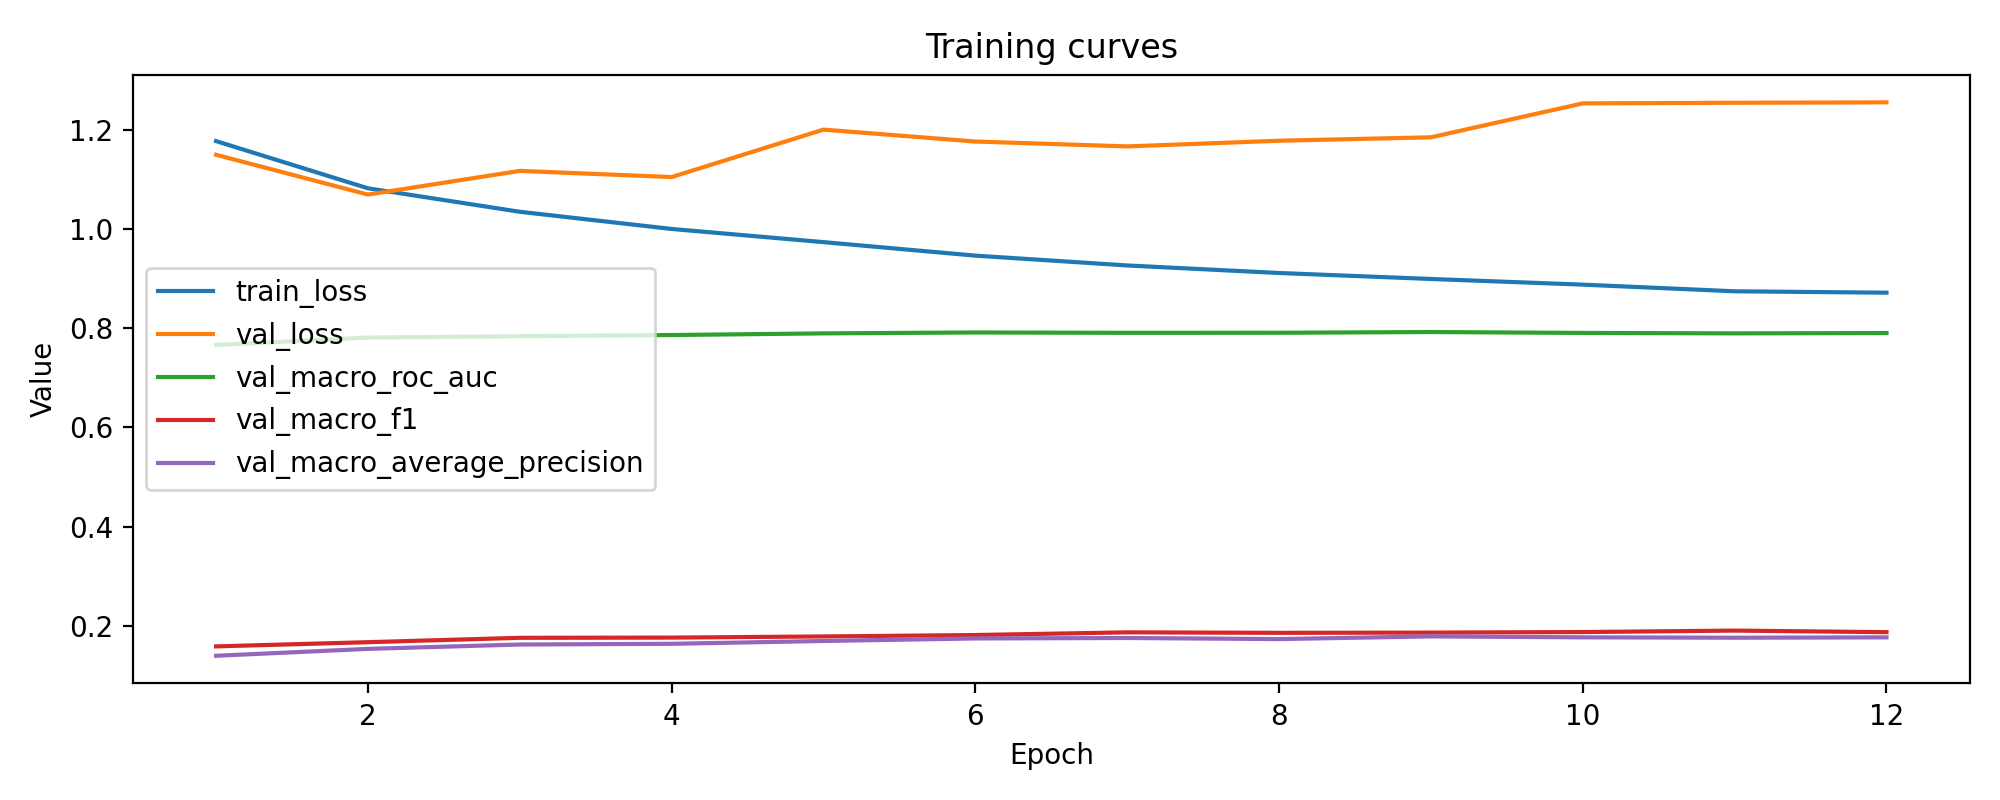
\includegraphics[width=0.82\textwidth]{../artifacts/supervised/resnet18_partial_finetune_224/training_curves.png}
    \caption{Courbes d'entra\^\i nement du meilleur run supervis\'e ResNet18 partial FT 224.}
\end{figure}

\begin{figure}[H]
    \centering
    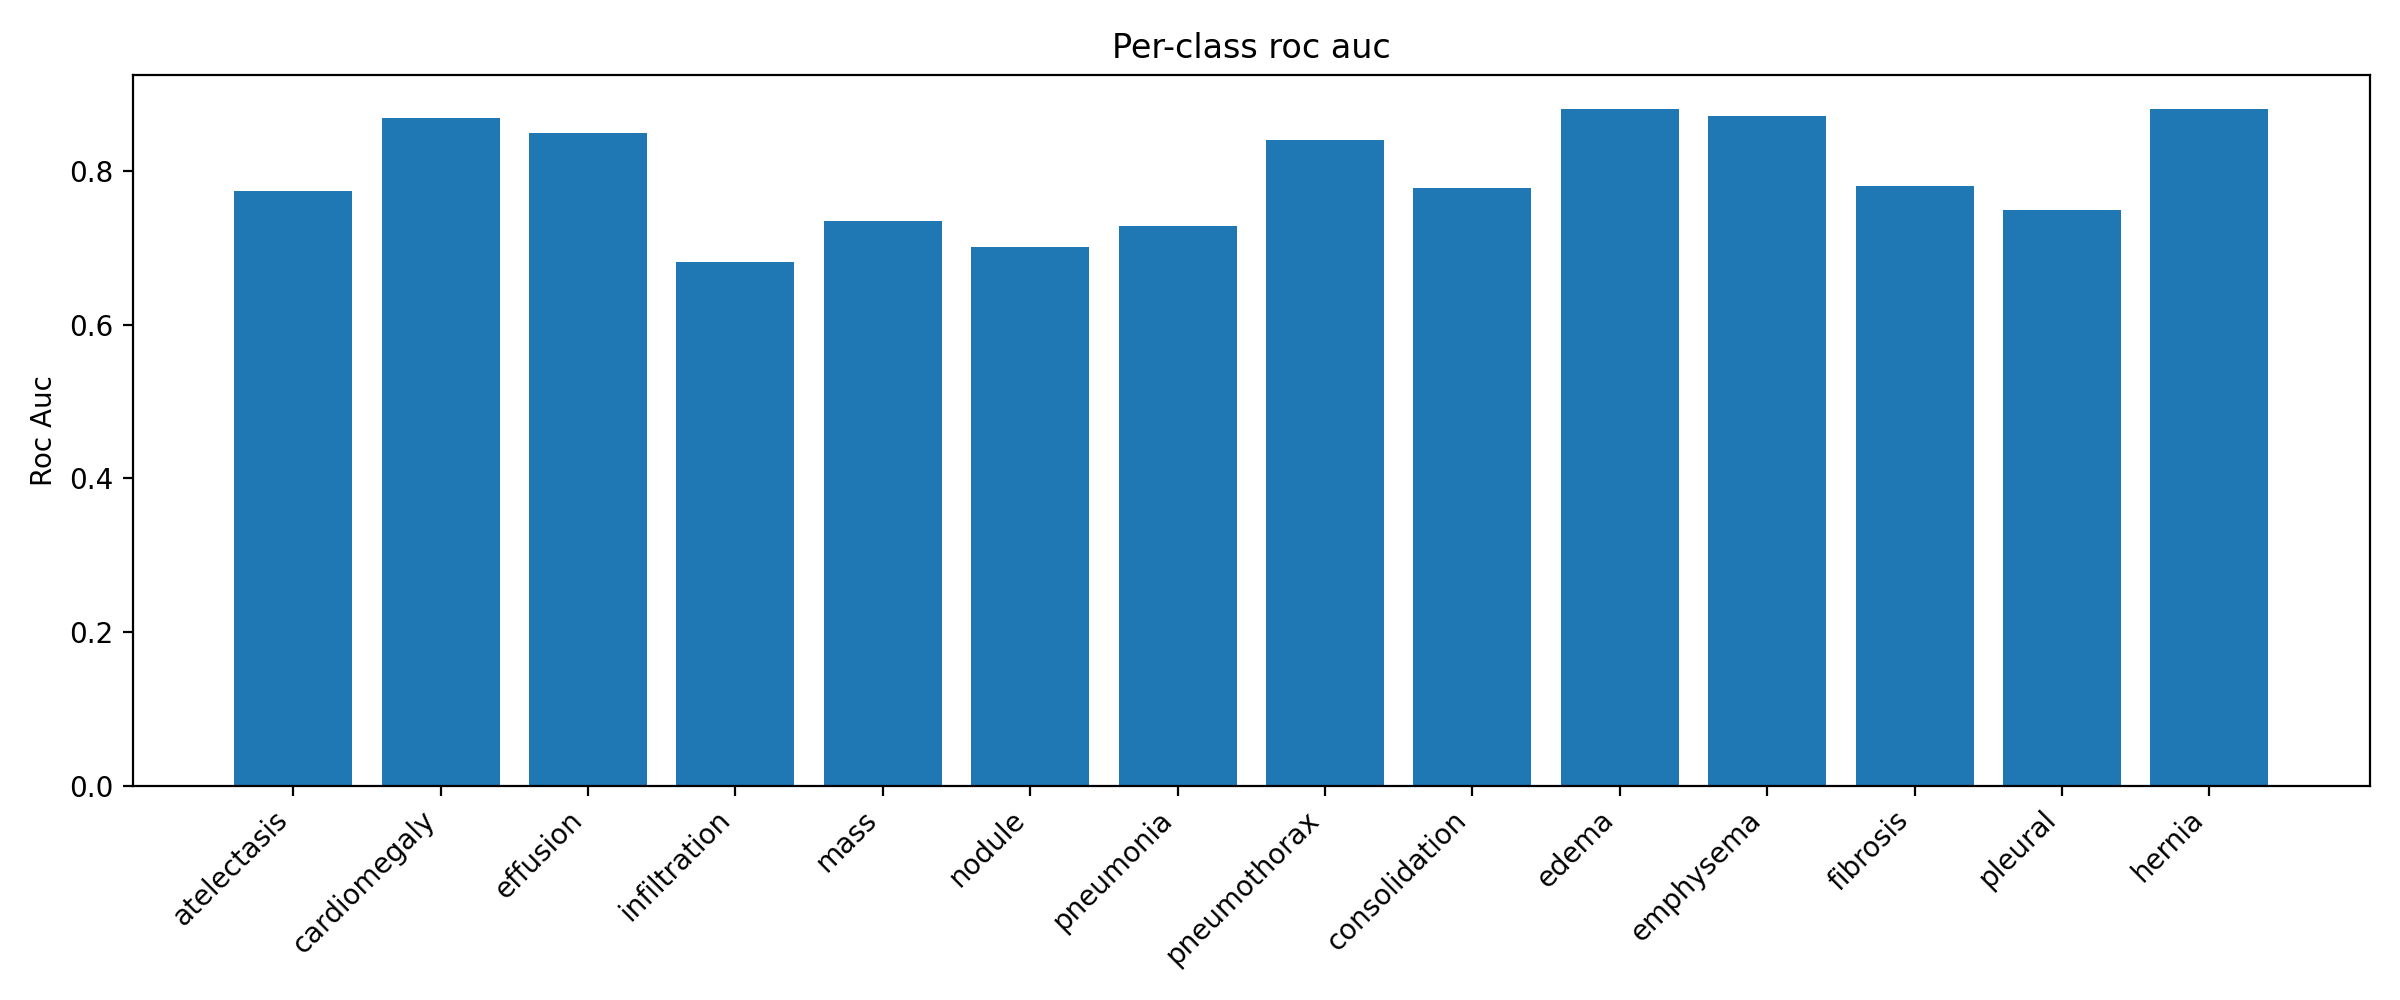
\includegraphics[width=0.82\textwidth]{../artifacts/supervised/resnet18_partial_finetune_224/per_class_roc_auc.png}
    \caption{ROC-AUC par classe pour le meilleur run supervis\'e ResNet18 partial FT 224.}
\end{figure}

\begin{figure}[H]
    \centering
    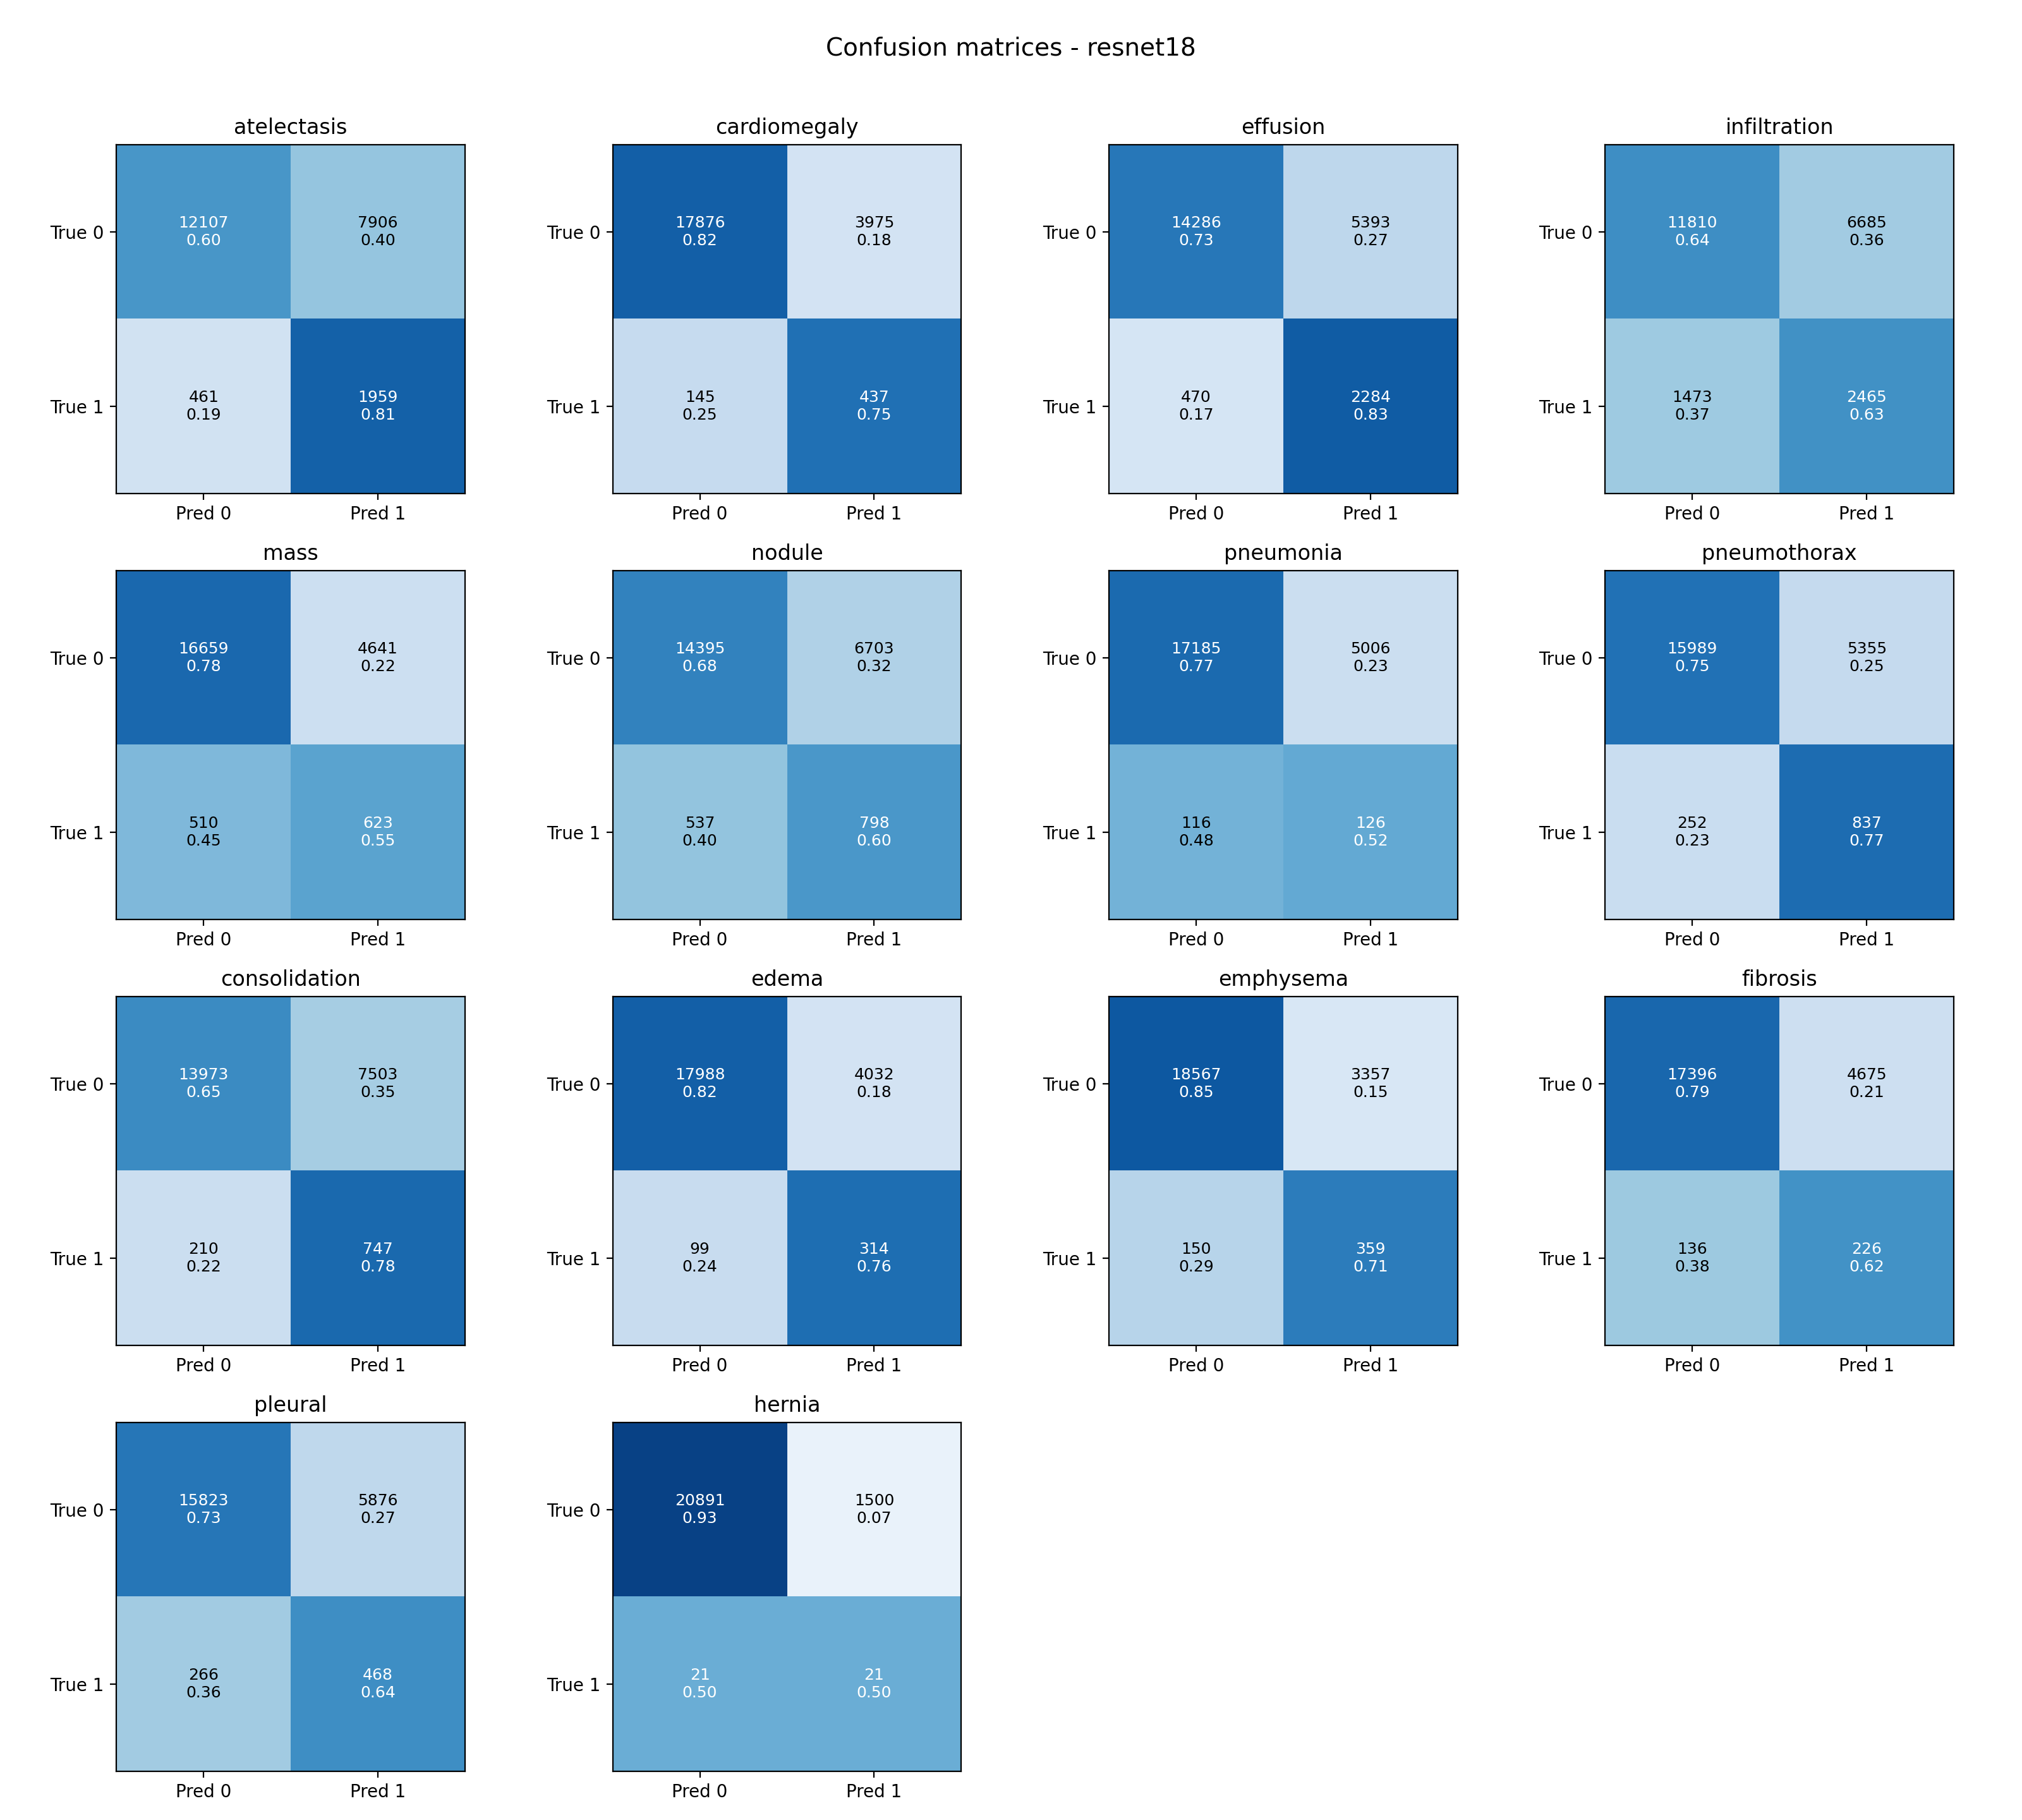
\includegraphics[width=0.90\textwidth]{../artifacts/supervised/resnet18_partial_finetune_224/confusion_matrix.png}
    \caption{Matrices de confusion par classe pour le meilleur run supervis\'e ResNet18 partial FT 224.}
\end{figure}

\subsection{Lecture finale de la brique d'anomalie}
Le run final de \textbf{Conv Autoencoder} atteint un ROC-AUC test de 0.4800, une Average Precision de 0.4534 et un F1 de 0.0840. Sous cette d\'efinition de l'anomalie, la s\'eparation entre cas normaux et cas pathologiques n'est donc pas satisfaisante. La m\'etrique de classement est m\^eme l\'eg\`erement inf\'erieure au hasard, ce qui indique que l'erreur de reconstruction ne constitue pas ici un proxy robuste de la pr\'esence d'une pathologie.

Ce r\'esultat n'invalide pas l'int\'er\^et de la d\'emarche, mais il en pr\'ecise clairement les limites. Plusieurs facteurs peuvent l'expliquer: la d\'efinition tr\`es large de ce qu'est une anomalie, le fait que certaines pathologies restent visuellement proches des cas normaux \`a basse r\'esolution, et la capacit\'e de l'autoencodeur \`a reconstruire aussi des motifs anormaux simples. Dans le cadre du projet, la brique anomalie doit donc \^etre pr\'esent\'ee comme un \textbf{signal exploratoire de vigilance} plut\^ot que comme un d\'etecteur fiable de pathologies.

\begin{figure}[H]
    \centering
    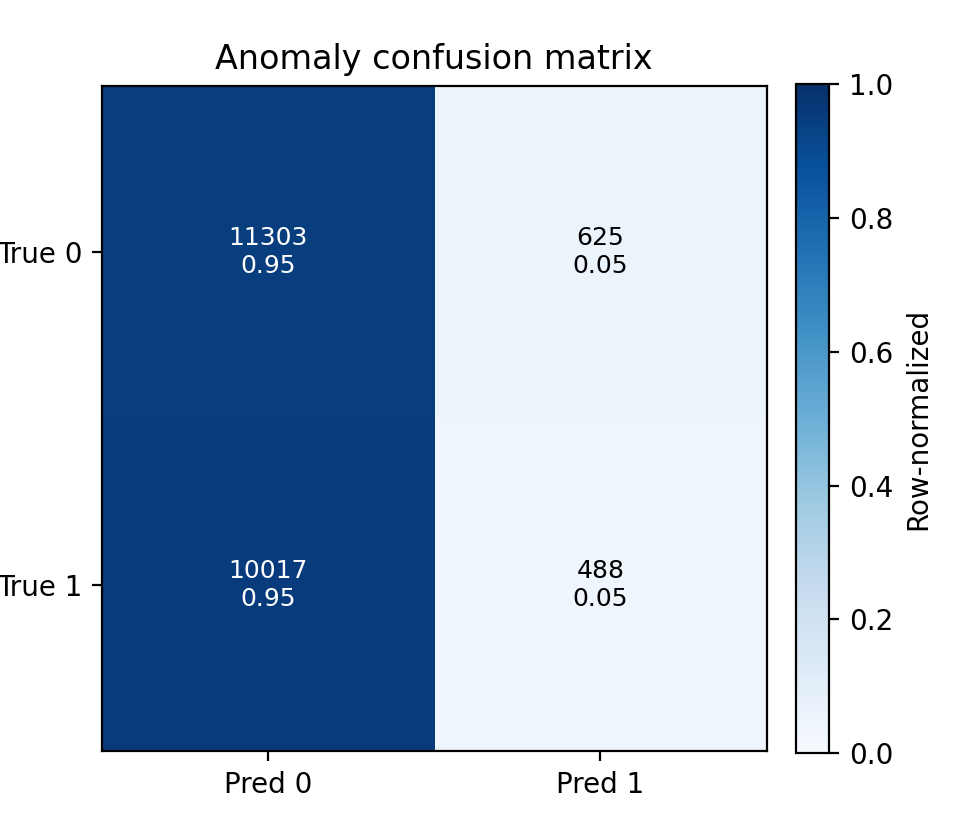
\includegraphics[width=0.56\textwidth]{../artifacts/anomaly/conv_autoencoder/confusion_matrix.png}
    \caption{Matrice de confusion binaire de la brique anomalie au seuil calibr\'e.}
\end{figure}

\subsection{Lecture finale des runs multimodaux}
Les r\'esultats multimodaux sont maintenant complets et tr\`es instructifs. La branche \textbf{image only} obtient un ROC-AUC macro de 0.5663, une AP macro de 0.1463 et un F1 macro de 0.1726. La branche \textbf{text only} atteint au contraire un ROC-AUC macro de 0.9953, une AP macro de 0.9823 et un F1 macro de 0.9445. La \textbf{fusion image + texte} obtient le meilleur score absolu avec un ROC-AUC macro de 0.9967, une AP macro de 0.9881 et un F1 macro de 0.9583.

La lecture de ces chiffres doit cependant rester tr\`es prudente. Le gain de la fusion sur le texte seul existe, mais il reste faible en valeur absolue. Surtout, le test de robustesse montre que lorsque le texte est supprim\'e, le ROC-AUC macro du mod\`ele de fusion chute \`a 0.5480, alors que lorsqu'on retire l'image il reste \`a 0.9966. Autrement dit, dans la configuration actuelle, le mod\`ele de fusion d\'epend presque enti\`erement de la modalit\'e textuelle.

Ce comportement est coh\'erent avec la construction du dataset IU X-Ray dans le projet. Les labels y sont des \emph{weak labels} extraits du texte, ce qui cr\'ee un lien direct entre la modalit\'e textuelle et la cible. Le rapport peut donc conclure que la multimodalit\'e est \textbf{fonctionnelle techniquement} et que la fusion obtient le meilleur score, mais il doit aussi souligner honn\^etement que cette sup\'eriorit\'e refl\`ete en grande partie la richesse de la modalit\'e texte et le mode de construction des labels, davantage qu'un apport massif de l'image.

\subsection{Snapshot final complet}
Le snapshot MLflow int\'egr\'e au rapport ne contient plus de cellules \emph{n.d.} pour les sept runs finaux attendus. Cette compl\'etude renforce la solidit\'e de la comparaison finale, puisque les conclusions reposent d\'esormais sur des runs r\'eellement termin\'es, trac\'es et sauvegard\'es, et non sur des r\'esultats interm\'ediaires ou des quickstarts.

\subsection{Analyse par classe et implications}
L'analyse par classe permet d'identifier plusieurs profils de difficult\'e. Les classes tr\`es rares comme \texttt{hernia} souffrent d'abord d'un probl\`eme de support statistique. Les classes plus fr\'equentes mais h\'et\'erog\`enes comme \texttt{infiltration} ou \texttt{mass} posent un autre type de difficult\'e: leur ph\'enotype radiologique est moins homog\`ene et donc plus difficile \`a capturer avec un mod\`ele compact.

Ces profils ont des cons\'equences pratiques sur le tri. Une classe \`a bon ROC-AUC mais faible F1 peut encore \^etre utile comme indicateur de priorit\'e si le syst\`eme est utilis\'e pour classer les examens par risque plut\^ot que pour produire une d\'ecision dure. En revanche, si l'on souhaite d\'eployer un seuil op\'erationnel unique, une calibration sp\'ecifique par classe devient presque indispensable.

\section{Tracking MLflow et tra\c{c}abilit\'e}
La tra\c{c}abilit\'e est assur\'ee avec MLflow, qui enregistre pour chaque run:
\begin{itemize}
    \item les hyperparam\`etres aplatis \`a partir des fichiers YAML;
    \item les m\'etriques par \'epoque et les scores de test;
    \item les figures de courbes, histogrammes, reconstructions, barplots et matrices de confusion;
    \item le meilleur checkpoint sauvegard\'e localement et journalis\'e comme artefact.
\end{itemize}

Les exp\'eriences sont structur\'ees en au moins trois exp\'eriences MLflow:
\begin{itemize}
    \item \texttt{chestmnist\_supervised};
    \item \texttt{chestmnist\_anomaly};
    \item \texttt{radiology\_multimodal}.
\end{itemize}

La coh\'erence entre entra\^\i nement et d\'eploiement est assur\'ee par le fait que l'application Streamlit recharge directement les checkpoints \texttt{best\_model.pt}, \texttt{best\_autoencoder.pt} et \texttt{best\_multimodal\_model.pt} produits par les scripts d'entra\^\i nement. L'application n'utilise donc pas des poids diff\'erents de ceux sauvegard\'es pendant le suivi exp\'erimental.

\subsection{Organisation pratique des runs}
Chaque famille d'exp\'eriences poss\`ede son propre espace logique, ses propres configurations YAML et son propre dossier d'artefacts. Cette organisation a plusieurs avantages. Elle simplifie la comparaison entre runs apparent\'es, elle \'evite de m\'elanger les checkpoints, et elle facilite la justification du ``meilleur mod\`ele retenu'' dans le rapport final.

Du point de vue m\'ethodologique, cette structure fait aussi gagner du temps \`a l'\'equipe. Lorsqu'un run produit un comportement inattendu, il est possible de remonter rapidement \`a la configuration r\'esolue, au type de normalisation, au nombre d'\'epoques effectivement parcourues, \`a la dur\'ee totale du run et aux figures sauvegard\'ees. MLflow ne sert donc pas uniquement \`a montrer des courbes en fin de projet; il sert aussi de journal de bord technique pendant tout le d\'eveloppement.

\subsection{Artefacts suivis}
\begin{table}[H]
    \centering
    \caption{Principaux artefacts suivis dans MLflow selon la famille de run.}
    \small
    \begin{tabular}{p{3.4cm}p{8.2cm}}
        \toprule
        Famille de run & Artefacts enregistr\'es \\
        \midrule
        Supervision & configuration r\'esolue, checkpoint meilleur mod\`ele, courbes d'entra\^\i nement, ROC-AUC par classe, AP par classe, matrices de confusion et m\'etriques test \\
        Anomalie & configuration r\'esolue, meilleur autoencodeur, courbes d'entra\^\i nement, histogramme des scores, grille de reconstructions, matrice de confusion et m\'etriques test \\
        Multimodal & configuration r\'esolue, meilleur mod\`ele, courbes d'entra\^\i nement, ROC-AUC par classe, matrices de confusion, robustesse \`a modalit\'e manquante et m\'etriques test \\
        \bottomrule
    \end{tabular}
\end{table}

\begin{figure}[htbp]
    \centering
    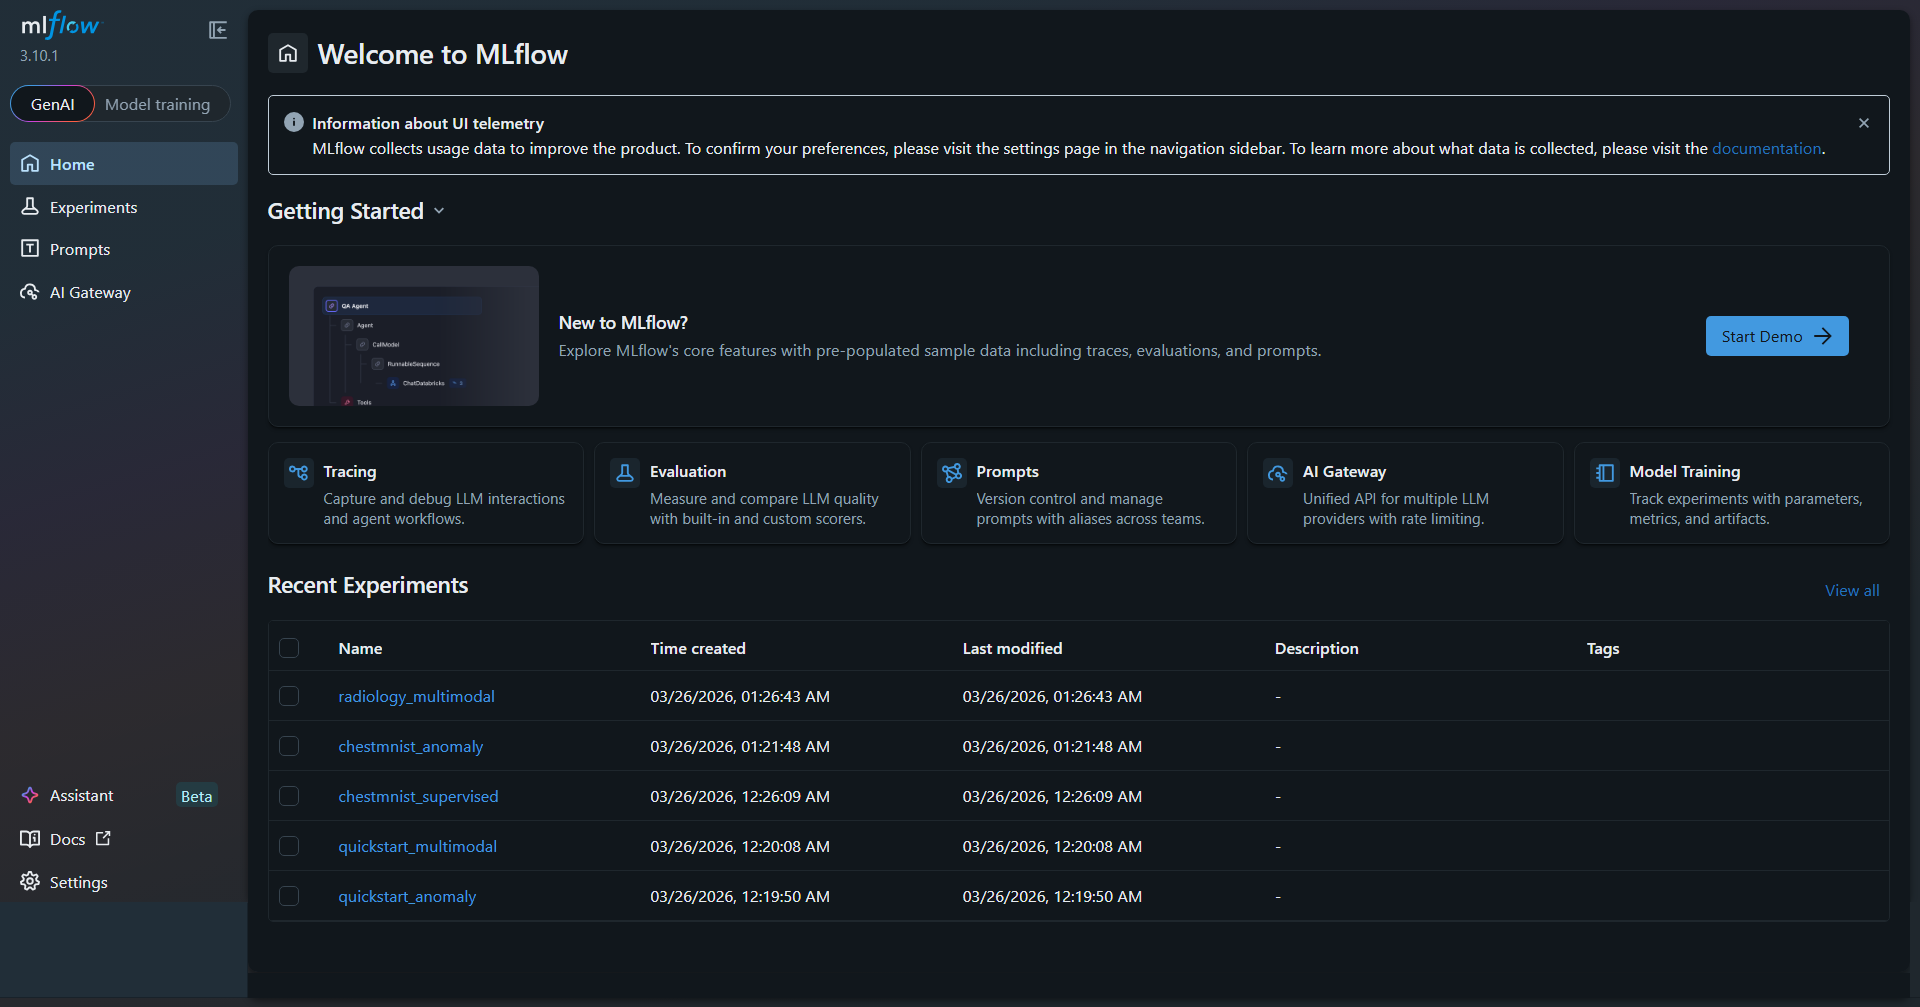
\includegraphics[width=0.92\textwidth]{../artifacts/screencapture-127-0-0-1-5000-2026-03-26-12_33_42.png}
    \caption{Capture d'\'ecran de l'interface MLflow locale utilis\'ee pour suivre les exp\'eriences du projet. On y retrouve les exp\'eriences principales, la navigation entre runs et l'acc\`es aux m\'etriques, param\`etres et artefacts.}
    \label{fig:mlflow-ui}
\end{figure}

\subsection{Tra\c{c}abilit\'e jusqu'au d\'eploiement}
L'un des points les plus importants du sujet est la coh\'erence entre le mod\`ele retenu et le mod\`ele effectivement expos\'e dans l'application. Dans ce projet, cette coh\'erence est assur\'ee par conception: Streamlit recharge les checkpoints finaux sauvegard\'es par les scripts d'entra\^\i nement, avec leur configuration, leurs labels et, pour la multimodalit\'e, leur vocabulaire. Le d\'emonstrateur pointe d\'esormais par d\'efaut vers \textbf{ResNet18 partial FT 224} pour la supervision, \textbf{Conv Autoencoder} pour l'anomalie et \textbf{Fusion IU X-Ray} pour la multimodalit\'e.

Pour rendre cette correspondance explicite et auditabile, un manifest de d\'eploiement est g\'en\'er\'e dans \texttt{artifacts/deployment\_manifest.json}. Il associe chaque checkpoint expos\'e dans l'application \`a son exp\'erience MLflow, \`a son \texttt{run\_name} et \`a son \texttt{run\_id}. Le tableau de tra\c{c}abilit\'e ins\'er\'e automatiquement dans le rapport reprend ces informations et constitue la preuve que les mod\`eles affich\'es dans la d\'emo correspondent bien \`a des runs trac\'es.

Cette continuit\'e est pr\'ecieuse d'un point de vue acad\'emique. Elle permet de d\'emontrer que le d\'emonstrateur n'est pas une interface d\'ecorr\'el\'ee du reste du travail, mais bien l'extension applicative du pipeline exp\'erimental.

\section{D\'emonstrateur applicatif}
Le prototype applicatif est impl\'ement\'e avec Streamlit \cite{streamlitdocs}. L'utilisateur peut charger une radiographie thoracique, obtenir:
\begin{itemize}
    \item les pr\'edictions supervis\'ees les plus probables;
    \item un score d'anomalie avec seuil et statut textuel;
    \item une pr\'ediction multimodale si un texte est fourni.
\end{itemize}

L'architecture de l'application est volontairement simple: chaque composant charge son checkpoint, son pr\'etraitement et, pour la branche multimodale, son vocabulaire. Cette s\'eparation rend le prototype plus lisible et facilite la maintenance.

Les limites du d\'emonstrateur sont cependant claires:
\begin{itemize}
    \item absence de serveur de production;
    \item absence de gestion fine des erreurs et de l'authentification;
    \item visualisation centr\'ee sur la pr\'ediction, sans explication clinique profonde;
    \item d\'ependance aux checkpoints disponibles localement.
\end{itemize}

\subsection{Architecture logicielle de l'application}
Le d\'emonstrateur s'appuie sur une logique modulaire. Trois bundles peuvent \^etre charg\'es s\'epar\'ement:
\begin{itemize}
    \item un bundle supervis\'e avec mod\`ele, transformations et noms de labels;
    \item un bundle anomalie avec autoencodeur, transformations et seuil;
    \item un bundle multimodal avec mod\`ele, vocabulaire, transformations et labels.
\end{itemize}

Cette architecture pr\'esente deux avantages majeurs. D'une part, chaque brique peut \^etre remplac\'ee sans casser les autres. D'autre part, l'application peut fonctionner m\^eme si tous les runs finaux ne sont pas encore disponibles, ce qui est tr\`es utile pendant la phase de d\'eveloppement du projet.

\subsection{Sc\'enario d'usage}
Du point de vue utilisateur, le parcours est volontairement simple. L'utilisateur charge une image thoracique, consulte les probabilit\'es des pathologies les plus probables, visualise le score d'anomalie et, s'il dispose d'un texte, peut comparer l'effet de la modalit\'e suppl\'ementaire. Ce sc\'enario est coh\'erent avec un usage de tri ou de d\'emonstration en cours, dans lequel un interne, un enseignant ou un \'etudiant veut voir rapidement comment plusieurs briques IA r\'eagissent sur le m\^eme examen.

Le prototype ne cherche pas \`a simuler un environnement hospitalier complet. Il s'agit d'une interface de test locale. Ce positionnement est assum\'e et coh\'erent avec la nature du projet: l'objectif est de rendre les mod\`eles manipulables et comparables, pas de livrer un logiciel m\'edical certifiable.

\begin{figure}[htbp]
    \centering
    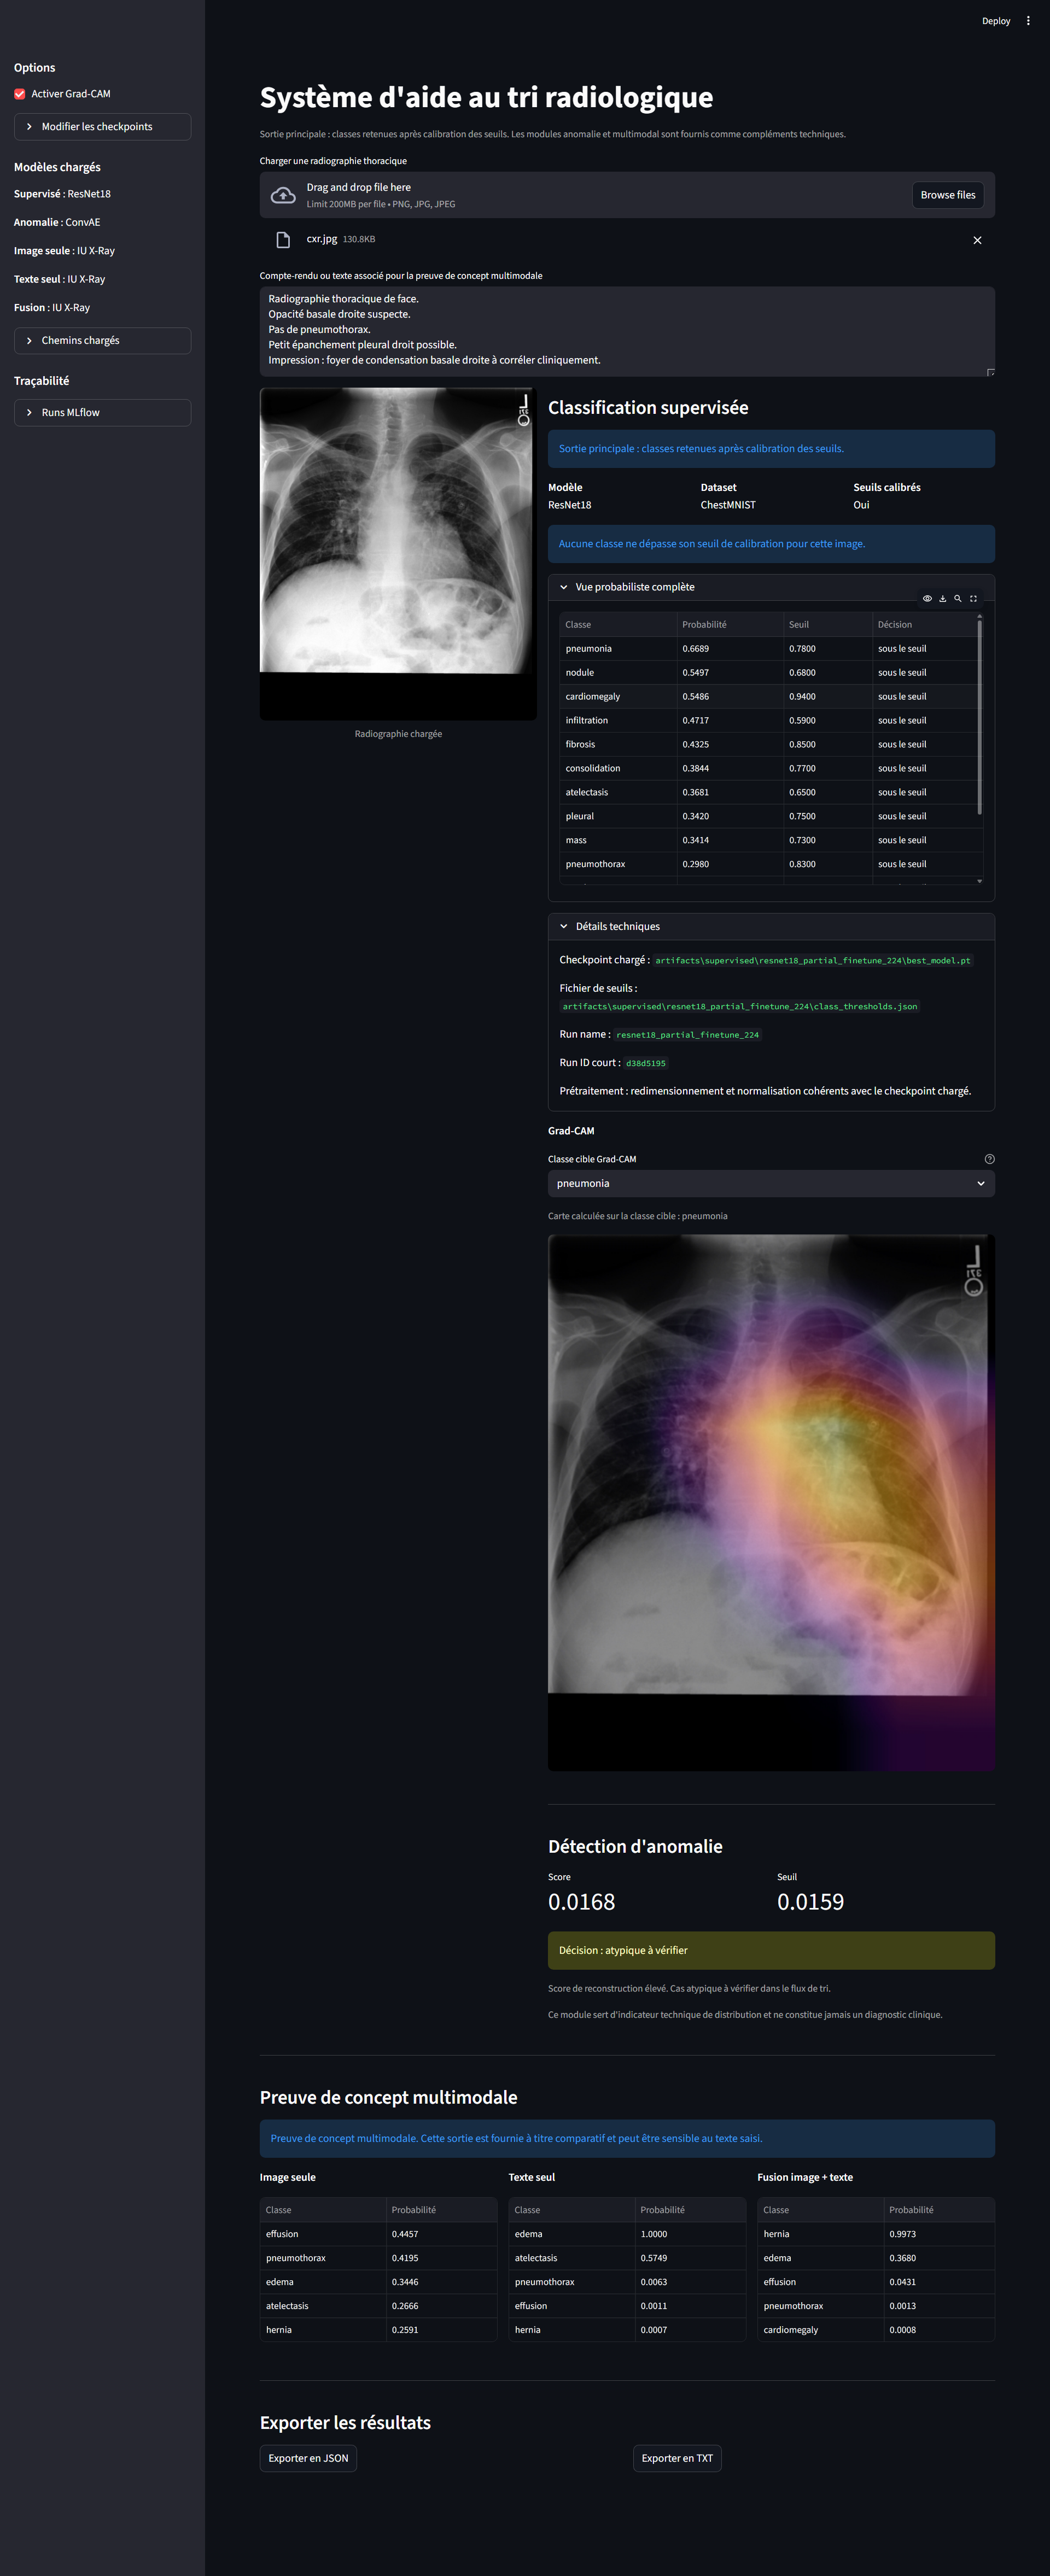
\includegraphics[width=0.56\textwidth]{../artifacts/screencapture-127-0-0-1-8501-2026-03-26-12_23_49.png}
    \caption{Capture d'\'ecran du d\'emonstrateur Streamlit final. L'interface rassemble la sortie supervis\'ee principale, le score d'anomalie, une visualisation Grad-CAM optionnelle et le module multimodal utilis\'e \`a titre comparatif.}
    \label{fig:streamlit-demo}
\end{figure}

\subsection{Limites applicatives et perspectives}
Si le projet devait \^etre prolong\'e au-del\`a du cadre acad\'emique, plusieurs extensions seraient naturelles: ajout d'explications visuelles de type cartes de saillance, historique des pr\'edictions, journalisation des inf\'erences, gestion de plusieurs utilisateurs, validation des formats DICOM et packaging applicatif plus robuste. Ces pistes d\'epassent le p\'erim\`etre initial, mais elles montrent que la base actuelle est compatible avec une mont\'ee en maturit\'e.

\section{Analyse critique}
Plusieurs enseignements ressortent du projet.

Premi\`erement, la partie supervis\'ee montre qu'un \textbf{transfer learning adapt\'e} constitue finalement la meilleure base du projet. Le run \textbf{ResNet18 partial FT 224} surpasse \textbf{SimpleCNN}, \textbf{ResNet18 transfer} \`a backbone gel\'e et \textbf{TinyViT}. Ce r\'esultat sugg\`ere qu'un backbone pr\'e-entra\^\i n\'e peut apporter un vrai gain \`a condition d'autoriser une adaptation partielle au domaine cible. La progression du F1 apr\`es calibration rappelle toutefois que le probl\`eme n'est pas r\'eduit \`a un simple classement; il reste fortement sensible au choix des seuils et au d\'es\'equilibre des classes.

Deuxi\`emement, la d\'etection d'anomalies par reconstruction reste pertinente conceptuellement pour signaler des cas atypiques, mais le run final montre aussi ses limites tr\`es clairement. Avec un ROC-AUC test voisin de 0.48, l'autoencodeur ne parvient pas \`a distinguer de mani\`ere fiable les images normales et pathologiques selon la d\'efinition retenue. Dans le projet, cette brique doit donc \^etre pr\'esent\'ee comme une preuve de concept technique et non comme un module de d\'ecision robuste.

Troisi\`emement, la multimodalit\'e apporte un int\'er\^et fort pour l'analyse radiologique, mais elle doit \^etre mani\'ee avec rigueur. Le fait que \textbf{text only} et \textbf{fusion} atteignent des scores presque parfaits, tandis que la suppression du texte fait chuter fortement la performance, confirme qu'une part essentielle du signal provient de la modalit\'e textuelle et du mode de construction des weak labels. Le choix d'une fusion interm\'ediaire et d'un test de robustesse \`a modalit\'e manquante permet justement de discuter cet aspect au-del\`a d'un simple score final.

Enfin, le compromis performance / co\^ut de calcul a \'et\'e central tout au long du projet. Une machine de type portable gamer avec RTX 2070 Max-Q permet de lancer le pipeline final, mais impose des arbitrages: taille d'image mod\'er\'ee, batch size raisonnable, backbone fig\'e en transfer learning, et Vision Transformer compact plut\^ot qu'un ViT lourd pr\'e-entra\^\i n\'e.

\subsection{Lecture d'ensemble des r\'esultats}
Le projet met en \'evidence une tension classique en imagerie m\'edicale: ce qui est facile \`a bien classer n'est pas toujours ce qui est le plus important cliniquement, et ce qui est important cliniquement est souvent rare, ambigu ou co-occurrent avec d'autres signes. La valeur du pipeline ne vient donc pas d'un seul chiffre de test, mais de la combinaison de plusieurs sorties: probabilit\'es supervis\'ees, score d'anomalie, robustesse multimodale et visualisation dans l'application.

Cette lecture syst\'emique est importante, car elle refl\`ete mieux l'esprit du sujet. Un bon projet ne consiste pas seulement \`a obtenir le meilleur score sur un benchmark; il consiste \`a articuler plusieurs briques compl\'ementaires de mani\`ere coh\'erente et tra\c{c}able.

\subsection{Robustesse et g\'en\'eralisation}
La question de la g\'en\'eralisation reste ouverte. Les datasets utilis\'es sont publics, de provenance limit\'ee et d\'ej\`a fortement pr\'e-trait\'es dans le cas de ChestMNIST. Il serait donc abusif d'extrapoler les performances \`a un autre h\^opital, \`a d'autres protocoles d'acquisition ou \`a d'autres populations sans exp\'erience suppl\'ementaire.

La branche anomalie apporte ici un int\'er\^et conceptuel: elle peut servir de filet de s\'ecurit\'e lorsque l'image semble sortir du domaine appris. Ce n'est pas une garantie de g\'en\'eralisation, mais c'est un pas vers une meilleure prudence syst\`eme.

\subsection{Biais, limites et pr\'ecautions d'interpr\'etation}
Plusieurs biais doivent \^etre explicitement rappel\'es dans la version finale du rapport. Le premier est le biais de classe: certaines pathologies rares ont trop peu d'exemples pour produire des estimations tr\`es stables. Le deuxi\`eme est le biais de source: les datasets utilis\'es ne repr\'esentent pas toute la vari\'et\'e de la radiologie thoracique r\'eelle. Le troisi\`eme est le biais de construction des labels multimodaux sur IU X-Ray, puisque ceux-ci sont extraits du texte lui-m\^eme.

Ce troisi\`eme point est sans doute le plus sensible. Il ne remet pas en cause l'int\'er\^et du pipeline multimodal comme preuve de concept, mais il impose de pr\'esenter les r\'esultats avec honn\^etet\'e. Si le mod\`ele texte seul s'av\`ere tr\`es fort, il faudra expliquer qu'une partie de cette force vient du lien direct entre la modalit\'e textuelle et les weak labels, et non d'une ``compr\'ehension clinique'' \`a proprement parler.

\subsection{Int\'er\^et p\'edagogique et scientifique du projet}
Malgr\'e ces limites, le projet conserve un int\'er\^et acad\'emique fort. Il oblige \`a traiter des probl\`emes r\'eels de donn\'ees, d'architecture, de protocole, de tra\c{c}abilit\'e, d'interface et d'interpr\'etation. Il montre aussi qu'un projet de deep learning m\'edical n'est pas r\'eduit au choix d'un backbone. La qualit\'e de la pr\'eparation des donn\'ees, de l'\'evaluation et de la coh\'erence logicielle compte au moins autant que la sophistication du mod\`ele.

\subsection{Enjeux \'ethiques et usage responsable}
Un syst\`eme d'aide au tri radiologique touche indirectement \`a des enjeux sensibles: priorit\'e des patients, risque de faux n\'egatifs, surconfiance dans l'IA et difficult\'e \`a expliquer certaines sorties. M\^eme dans un cadre de projet, il est important de rappeler qu'aucune pr\'ediction du pipeline ne doit \^etre interpr\'et\'ee comme un avis m\'edical autonome.

Cette prudence est d'ailleurs coh\'erente avec le design du d\'emonstrateur: l'application affiche des scores et des messages de vigilance, mais ne pr\'esente jamais la sortie comme une d\'ecision d\'efinitive. Une telle posture est indispensable si l'on veut discuter l'usage responsable de l'apprentissage profond en sant\'e.

\section{Conclusion et perspectives}
Le projet aboutit \`a une base coh\'erente de syst\`eme d'aide au tri radiologique combinant classification supervis\'ee, d\'etection d'anomalies, multimodalit\'e, tra\c{c}abilit\'e MLflow et d\'emonstrateur Streamlit. Au vu des r\'esultats finaux, la solution la plus raisonnable \`a recommander \`a ce stade est le couple:
\begin{itemize}
    \item \textbf{ResNet18 partial FT 224} comme mod\`ele supervis\'e principal recommand\'e sur ChestMNIST, avec calibration de seuils par classe;
    \item une brique d'anomalie conserv\'ee comme module exploratoire de vigilance, mais pas comme signal d\'ecisionnel fort;
    \item une branche multimodale utilis\'ee comme enrichissement contextuel et comme preuve de concept, avec une lecture prudente des performances \`a cause des weak labels textuels.
\end{itemize}

Les perspectives d'am\'elioration les plus naturelles sont:
\begin{itemize}
    \item calibrer les seuils par classe pour am\'eliorer le F1 des mod\`eles supervis\'es;
    \item tester un fine-tuning partiel ou complet du backbone de transfer learning, voire un backbone pr\'e-entra\^\i n\'e en imagerie m\'edicale;
    \item remplacer le GRU texte par un encodeur biom\'edical pr\'e-entra\^\i n\'e;
    \item reconstruire la partie multimodale sur des labels ind\'ependants du texte ou sur des annotations plus directement valid\'ees;
    \item approfondir la partie anomalie avec un VAE ou une approche d'\'energie;
    \item enrichir l'application avec explications visuelles et export de rapport.
\end{itemize}

En l'\'etat, le projet constitue une base acad\'emique solide, reproductible et extensible pour discuter les enjeux d'un syst\`eme de tri radiologique assist\'e par apprentissage profond.

\clearpage
\begin{thebibliography}{9}

\bibitem{yang2023medmnist}
Jiancheng Yang, Rui Shi, Donglai Wei, Zequan Liu, Lin Zhao, Bilian Ke, Hanspeter Pfister et Bingbing Ni.
\newblock MedMNIST v2 - A large-scale lightweight benchmark for 2D and 3D biomedical image classification.
\newblock \emph{Scientific Data}, 10:41, 2023.
\newblock DOI: \href{https://doi.org/10.1038/s41597-022-01721-8}{10.1038/s41597-022-01721-8}.

\bibitem{wang2017chestxray8}
Xiaosong Wang, Yifan Peng, Le Lu, Zhiyong Lu, Mohammadhadi Bagheri et Ronald M. Summers.
\newblock ChestX-ray8: Hospital-Scale Chest X-Ray Database and Benchmarks on Weakly-Supervised Classification and Localization of Common Thorax Diseases.
\newblock In \emph{Proceedings of the IEEE Conference on Computer Vision and Pattern Recognition (CVPR)}, 2017.
\newblock URL: \href{https://openaccess.thecvf.com/content_cvpr_2017/papers/Wang_ChestX-ray8_Hospital-Scale_Chest_CVPR_2017_paper.pdf}{openaccess.thecvf.com}.

\bibitem{demnerfushman2016openi}
Dina Demner-Fushman, Marc D. Kohli, Marc B. Rosenman, Sonya E. Shooshan, Laritza Rodriguez, Sameer Antani, George R. Thoma et Clement J. McDonald.
\newblock Preparing a collection of radiology examinations for distribution and retrieval.
\newblock \emph{Journal of the American Medical Informatics Association}, 23(2):304--310, 2016.
\newblock DOI: \href{https://doi.org/10.1093/jamia/ocv080}{10.1093/jamia/ocv080}.

\bibitem{he2016resnet}
Kaiming He, Xiangyu Zhang, Shaoqing Ren et Jian Sun.
\newblock Deep Residual Learning for Image Recognition.
\newblock In \emph{Proceedings of the IEEE Conference on Computer Vision and Pattern Recognition (CVPR)}, 2016.
\newblock URL: \href{https://openaccess.thecvf.com/content_cvpr_2016/html/He_Deep_Residual_Learning_CVPR_2016_paper.html}{openaccess.thecvf.com}.

\bibitem{dosovitskiy2021vit}
Alexey Dosovitskiy, Lucas Beyer, Alexander Kolesnikov et al.
\newblock An Image is Worth 16x16 Words: Transformers for Image Recognition at Scale.
\newblock In \emph{International Conference on Learning Representations (ICLR)}, 2021.
\newblock URL: \href{https://arxiv.org/abs/2010.11929}{arxiv.org/abs/2010.11929}.

\bibitem{mlflowdocs}
MLflow.
\newblock MLflow Documentation.
\newblock URL: \href{https://mlflow.org/docs/latest/index.html}{mlflow.org/docs/latest/index.html}.

\bibitem{streamlitdocs}
Streamlit.
\newblock Streamlit Documentation.
\newblock URL: \href{https://docs.streamlit.io/}{docs.streamlit.io}.

\end{thebibliography}

\end{document}
